% \documentclass[12pt]{article}
\documentclass[12pt]{ctexart}
\usepackage[utf8]{inputenc}

\usepackage[english]{babel}
\usepackage[dvips]{epsfig}
\usepackage{amsmath}
\usepackage{amssymb}
\usepackage{amsfonts}
\usepackage{amsthm}
\usepackage{amsbsy}
\usepackage{amsgen}
\usepackage{amscd}
\usepackage{amsopn}
\usepackage{amstext}
\usepackage{amsxtra}
\usepackage{mathrsfs}
\usepackage{enumitem}
\usepackage{graphicx}
\usepackage{verbatim}
\usepackage{epstopdf}
\usepackage{float}
\usepackage[all,cmtip]{xy}
\usepackage{accents}
\usepackage{sseq}
\usepackage{url}
\usepackage{hyperref}
\usepackage{makeidx}
\usepackage{siunitx}
\usepackage{xcolor}
\usepackage{physics}

%%%%%%%%% 版面设置 %%%%%%%%%%%%%%%%%%%%%%%%%%%%%%%%%%%%%%
\usepackage{geometry}
\usepackage{titlesec}
\usepackage{fancyhdr}\pagestyle{empty}
\titleformat*{\section}{\large\bfseries}

%
\geometry{
	a4paper,
	total={170mm,240mm},
	left=20mm,
	top=30mm,
}

%Bitte nicht einstellen
\renewcommand{\figurename}{Abbildung}
\renewcommand{\tablename}{Tabelle}
\pagestyle{fancyplain}
\headheight 35pt
\lhead{\name}
\chead{\textbf{\Large \Title}}
\rhead{\due\\\today}
\lfoot{}
\cfoot{}
\rfoot{\small\thepage}
\headsep 1.5em

%%%%%%%%%%%%%%%%%%%%%%%%%%%%%%%%%%%%%%%%%%%%%%%%%%%%%%

\newtheorem{thm}{Theorem}[section]

% 定义解题环境
\theoremstyle{remark}
\newtheorem{remark}[thm]{Remark}
\newtheorem{theorem}{Theorem}
\newtheorem{observation}[thm]{Observation}

\theoremstyle{definition}
\newtheorem{problem}{\text{}}
\newtheorem{Problem}{\text{Problem}}
\newtheorem*{solution}{解}
\newtheorem*{Answer}{Answer}
\newtheorem{example}{Example} 

%%%%%%%%%%%%%%%%%%%%%%%%%%%%%%%%%%%%%%%%%%%%%%%%%%%%%%%%%%%%%%%%%%
\newcommand\name{陈景龙22120307}
\newcommand\due{-}
\newcommand{\emptyline}{\vspace{0.6\baselineskip}}


\newcommand\Title{智能计算数学基础笔记}
\renewcommand\due{due: November 6, 2022}
\newcommand\dom{\operatorname{dom}} % 定义域
\newcommand\diag{\operatorname{diag}} % 对角矩阵
\newcommand\epi{\operatorname{epi}} % 上镜图
\newcommand\minimize{\operatorname{minimize}} % 最小化
\newcommand\maximize{\operatorname{maximize}} % 最大化
\newcommand\subject{\operatorname{subject\ to}}
\newcommand\vc{\overrightarrow} % 向量符号

\usepackage{listings}

\lstset{
    basicstyle          =   \sffamily,          % 基本代码风格
    keywordstyle        =   \bfseries,          % 关键字风格
    commentstyle        =   \rmfamily\itshape,  % 注释的风格,斜体
    stringstyle         =   \ttfamily,  % 字符串风格
    flexiblecolumns,                % 别问为什么,加上这个
    numbers             =   left,   % 行号的位置在左边
    showspaces          =   false,  % 是否显示空格,显示了有点乱,所以不现实了
    numberstyle         =   \zihao{-5}\ttfamily,    % 行号的样式,小五号,tt等宽字体
    showstringspaces    =   false,
    captionpos          =   t,      % 这段代码的名字所呈现的位置,t指的是top上面
    frame               =   l,   % 显示边框
}
\lstdefinestyle{cpp}{
    language        =   C++, % 语言选C++
    basicstyle      =   \zihao{-5}\ttfamily,
    numberstyle     =   \zihao{-5}\ttfamily,
    keywordstyle    =   \color{blue}, % 彩色
    keywordstyle    =   [2] \color{teal},% 彩色
    % keywordstyle    =   \color{black}, % 黑白
    % keywordstyle    =   [2] \color{black},% 黑白
    stringstyle     =   \color{magenta}, % 彩色
    stringstyle     =   \color{black}, % 黑白
    commentstyle    =   \color{red}\ttfamily,% 彩色
    % commentstyle    =   \color{black}\ttfamily, % 黑白
    breaklines      =   true,   % 自动换行,建议不要写太长的行
    columns         =   fixed,  % 如果不加这一句,字间距就不固定,很丑,必须加
    basewidth       =   0.5em,
}


\begin{document}

% \maketitle
考核方式:出勤(10\%)+ 大作业(20\%) + 笔试(70\%)

\section{微积分}
\begin{remark}
    给定集合 $A \subset \mathbb{R}^n$\begin{itemize}
        \item 开集:对于任何$x \in A$都存在以 $x$ 为中心的开球 $B(x, r) = \left\{y \in \mathbb{R}^n: \norm{y - x} < r\right\}$ 使得 $B(x, r) \subset A$\begin{itemize}
            \item 任意个开集之并是开集,有限个开集之交是开集
        \end{itemize}
        \item 闭集:补集 $(\mathbb{R}^n - A)$ 是开集\begin{itemize}
            \item 任意个闭集之交是闭集,有限个闭集之并是闭集
            \item $A = \bar{A}$,即:如果 $\left\{x_k\right\}_{k \ge 1} \subset A,\underset{k \to \inf}{\lim}x_k = x$,则 $x \in A$
        \end{itemize}
        \item  紧集:$A$ 是一个有界闭集,即 $A$ 是闭集并且存在开球 $B(x, r)$ 使得 $A \subset B(x, r)$
    \end{itemize}
\end{remark}

\begin{remark}
    $f: D \mapsto \mathbb{R}, D \subset \mathbb{R}^n$ 开集,$a \in D$\begin{itemize}
        \item 偏导(方向导数的特例):$\partial_if(a) = \underset{t \to 0}{\lim}\frac{f(a + te_i) - f(a)}{t}$
        \item 梯度:$\nabla f(a) = (\partial_1f(a), \dots, \partial_nf(a))^t$
        \item 可微:如果存在向量 $v \in \mathbb{R}^n$ 使得\[\lim_{x \to a}\frac{|f(x) - f(a) - v^t(x - a)|}{\norm{x - a}} = 0\]此时,$v^t$ 称为 $a$ 点的微分,记作 $Df(Aa)$ 或者 $\frac{\partial f(a)}{\partial a}$
        \item $f$ 在 $a$ 点可微 $\Longleftrightarrow f(x) = f(a) + Df(a)(x - a) + o(\norm{x - a})$
        \item $f$ 在 $a$ 点可微 $\Longrightarrow f$ 在 $a$ 点连续、各个方向上存在偏导,$Df(a) = \nabla f(a)^t$\begin{itemize}
            \item $f(x) = f(a) + \nabla f(a)^t(x - a) + o(\norm{x - a})$
        \end{itemize} 
    \end{itemize}
\end{remark}

\begin{remark}
	$\norm{A}^2 = \tr(AA^t)$
\end{remark}

\begin{remark}
    $f: \mathbb{R}^{m \times n} \mapsto \mathbb{R}$,变量为 $m \times n$ 的矩阵 $A = (a_{i, j})$\begin{itemize}
        \item 按照上述定义,$Df(A) = (\partial_{a_{i, j}}f(A))$ 是一个长度为 $m \times n$ 的行向量
        \item 但是为了方便起见,通常将 $Df(A)$ 写成一个 $m \times n$ 的矩阵,其 $(i, j)$ 位置的元素 $\partial_{a_{i, j}}f(A)$,即 $(Df(A))_{i, j} = \partial_{a_{i, j}}f(A)$
    \end{itemize}
\end{remark}

\begin{remark}
	对于无约束优化问题 $\minimize\ f(x)$:
	\begin{itemize}
		\item $x^*$ 是局部极小值点的必要条件为 $\nabla f(x^*) = 0, \nabla^2f(x^*)\succeq 0$;
		\item $x^*$ 是局部极小值点的充分条件为 $\nabla f(x^*) = 0, \nabla^2f(x^*)\succ 0$;
		\item 如果 $f$ 是凸函数,$x^*$ 为极小值点的充要条件为 $\nabla f(x^*) = 0$;
		\item $f$ 是凸函数的充要条件为 $\nabla^2f\succeq 0$。
	\end{itemize}
\end{remark}

\begin{remark}
	对于等式约束($Ax=b, A\in \mathbb{R}^{p\times n}$)优化问题 $\minimize\ f(x)$:
	\begin{itemize}
		\item $x^*$ 是局部极小值点的必要条件为 $Ax^*=b, B^t\nabla f(x^*) = 0, B^t\nabla^2f(x^*)B \succeq 0$;
		\item $x^*$ 是局部极小值点的充分条件为 $Ax^*=b, B^t\nabla f(x^*) = 0, B^t\nabla^2f(x^*)B \succ 0$;
		\item 如果 $f$ 是凸函数,$x^*$ 为极小值点的充要条件为 $Ax^*=b, B^t\nabla f(x^*) = 0$。
		\item 其中 $B=(\alpha_1, \dots, \alpha_{n - p})$,$\left\{\alpha_1, \dots, \alpha_{n - p}\right\}$ 是 $\mathcal{N}(A)$ 的一组基;
		\item 使用拉格朗日乘子求解 $x^*$,再进行验证。
	\end{itemize}
\end{remark}

\section{线性代数}
\begin{remark}
    对于 $\mathbb{R}$ 上矩阵 $A_{m \times n}$
    \begin{itemize}
        \item 行向量构成 $\mathbb{R}^n$ 中的子空间
        \item 列向量构成 $\mathbb{R}^m$ 中的子空间
        \item $A$ 的列空间 $C(A) := \left\{Ax \mid x \in \mathbb{R}^n\right\}$,是所有列向量的线性组合\begin{itemize}
            \item 对 $A$ 列分块,$Ax$ 是 $A$ 的列向量的线性组合
            \item $A=\begin{bmatrix}
                \beta_{1} & \beta_{2} & \cdots & \beta_{n}
            \end{bmatrix}, C(A)=\left\{x_{1} \beta_{1}+\cdots + x_{n} \beta_{n} \mid x_{i} \in \mathbb{R}, \beta_i \in \mathbb{R}^m\right\}$
            \item 等于 $A$ 的映射的像 $\operatorname{Im}(A)$
            \item 是 $\mathbb{R}^m$ 的子空间
            \item $\dim C(A) = \rank A = r$
        \end{itemize}
        \item $A$ 的行空间\begin{itemize}
            \item 对 $A$ 行分块,$A = (\alpha_1^t\ \cdots\  \alpha_m^t)^t$
            \item 定义行空间 $\left\{y_1\alpha_1 + \cdots + y_m\alpha_m \mid y_i \in \mathbb{R}, \alpha_i \in \mathbb{R}^n\right\}$
            \item 等于 $A^T$ 的映射的像 $\operatorname{Im}(A^T)$
            \item 是 $\mathbb{R}^n$ 的子空间
            \item $\dim C(A^T) = \rank A^T = r$
        \end{itemize}
        \item $n = \dim \mathcal{N}(A) + \rank(A)$
    \end{itemize}
\end{remark}

\begin{remark}
    观察 $Ax = 0$
    \begin{itemize}
        \item 零空间 $\mathcal{N}(A)$ 中的元素 $x$ 与 $A$ 的每一行正交
        \item 零空间 $\mathcal{N}(A)$ 中的元素 $x$ 与 $A$ 的行空间正交 $x \perp C(A^T)$
        \item 若 $x$ 为行空间 $C(A^T)$ 中的非零元素(行向量线性组合),$Ax \neq 0$。
        \item $\mathcal{N}(A) \perp C(A^T), \mathcal{N}(A^T) \perp C(A)$,分别在 $\mathbb{R}^n$ 和 $\mathbb{R}^m$ 中互为正交补。
        \item $\mathcal{N}(A)$ 的维度为 $n - r$,$\mathcal{N}(A^T)$ 的维度为 $m - r$。
    \end{itemize}
\end{remark}

\begin{remark}
	$A^TA$ 的零空间等于 $A$ 的零空间:$\mathcal{N}(A^TA) = \mathcal{N}(A)$。
	\begin{itemize}
		\item $x\in\mathcal{N}(A) \Leftrightarrow Ax=0 \Rightarrow A^TAx=0 \Rightarrow x \in \mathcal{N}(A^TA)$
		\item $x \in \mathcal{N}(A^TA)\Leftrightarrow A^TAx = 0 \Rightarrow Ax \in \mathcal{N}(A^T) \Rightarrow Ax \in \mathcal{N}(A^T)\cap C(A)=\left\{0\right\} \Rightarrow x\in \mathcal{N}(A)$
	\end{itemize}
\end{remark}

\begin{remark}
	$A$ 的列向量线性无关,则 $A^TA$ 可逆。
	\begin{itemize}
		\item $A$ 的列向量线性无关 $\Rightarrow \mathcal{N}(A) = \left\{0\right\}\Rightarrow \mathcal{N}(A^TA) = \left\{0\right\}\Rightarrow A^TA$ 可逆。
	\end{itemize}
\end{remark}

\begin{remark}
    满足 $Q^TQ = I$ 的方阵 $Q$ 是一个正交方阵。
    \begin{itemize}
        \item 等距:$\norm{Qx}^2 = x^TQ^TQx = x^Tx = \norm{x}^2$
        \item 特征值的模长为 $1$:$Qx = \lambda x, \norm{Qx}^2 = \norm{x}^2\Rightarrow |\lambda|^2 = 1$
    \end{itemize}
\end{remark}

\begin{remark}
    正交方阵:
    \begin{itemize}
        \item 向量 $x$ 逆时针旋转 $\theta$ 角得到向量 $y = \begin{bmatrix}
            \cos\theta & -\sin\theta \\ 
            \sin\theta & \cos\theta
        \end{bmatrix}x$;
        \item 向量 $x$ 沿 $\theta/2$ 角对称得到向量 $y = \begin{bmatrix}
            \cos\theta & \sin\theta \\ 
            \sin\theta & -\cos\theta
        \end{bmatrix}x = \begin{bmatrix}
            \cos\theta & -\sin\theta \\ 
            \sin\theta & \cos\theta
        \end{bmatrix}\begin{bmatrix}
            1 & 0 \\
            0 & -1
        \end{bmatrix}x$;也就是先关于 $x$ 轴对称,再旋转 $\theta$ 度。
        \item 向量 $x$ 关于单位向量 $u$ 对称,得到向量 $y = (2uu^T-I)x$。
    \end{itemize}
\end{remark}

\begin{remark}
    $y$ 在 $x$ 上的投影向量为 \[\frac{x^{T} y}{\norm{x}} \cdot \frac{x}{\norm{x}}=\frac{x^{T} y}{x^{T} x} x=x \frac{x^{T} y}{x^{T} x}=\frac{x x^{T}}{x^{T} x} y\]
    \begin{itemize}
        \item $P = \frac{x x^{T}}{x^{T} x}$ 称为 $x$ 的投影矩阵
        \item 对任意 $\alpha$,$P\alpha$ 是 $\alpha$ 在 $x$ 上的投影
        \item $P$ 是对称的,$\rank(P) = 1, P^2 = P$
    \end{itemize}
\end{remark}

\begin{remark}
    $\left\{v_1, \dots, v_n\right\}$ 是 $V$ 的一组基,$S_{i, j} = \left\langle v_{i}, v_{j}\right\rangle$。则 $V$ 空间下的任意两个向量 $x, y$ 的内积 $\left\langle x, y\right\rangle=x^TSy$。当 $\left\langle v_{i}, v_{i}\right\rangle = 1, \left\langle v_{i}, v_{j}\right\rangle = 0$ 时,$S$ 为单位阵,内积变为 \[x^TSy = x_1y_1 + \cdots + x_ny_n\]
    此时 $\left\{v_i\right\}$ 是一组标准正交基。
\end{remark}

\begin{remark}
    Gram-Schmidt 正交化:\textbf{线性无关向量} $a_1, \dots, a_n$ 通过 Gram-Schmidt 正交化生成标准正交向量 $q_1, \dots, q_n$:
    \begin{align*}
        q_{1}= & a_{1} /|a_{1}| & & \\
        a_{2}^{\prime}= &a_{2}-q_{1} q_{1}^{T} a_{2}, & q_{2}=&a_{2}^{\prime} /|a_{2}^{\prime}| \\
        a_{3}^{\prime}= & a_{3}-q_{1} q_{1}^{T} a_{3}-q_{2} q_{2}^{T} a_{3}, & q_{3}=&a_{3}^{\prime} /|a_{3}^{\prime}| \\
        & \vdots & \vdots &
    \end{align*}

    \[\begin{bmatrix}
        a_{1} & \cdots & a_{n}
    \end{bmatrix}\begin{bmatrix}
        b_{11} & b_{12} & \cdots & b_{1 n} \\
        & b_{22} & \cdots & b_{2 n} \\
        & & \ddots & \vdots \\
        & & & b_{n n}
    \end{bmatrix}=\begin{bmatrix}
        q_{1} & \cdots & q_{n}
    \end{bmatrix}\]

    $A_{m\times n}$ 的列向量线性无关,通过 Gram-Schmidt 正交化:
    \[A_{m\times n}T_{n\times n} = Q_{m\times n}\]
    $T$ 为可逆上三角矩阵,$Q$ 的列向量标准正交。当 $m=n$ 时,$Q$ 是正交方阵。两边同时乘以 $T$ 的逆矩阵(上三角的逆矩阵还是上三角)
    \[A_{m \times n}=Q_{m \times n} R_{n \times n}=\begin{bmatrix}
        q_{1} & q_{n}
    \end{bmatrix}\begin{bmatrix}  
        &  & r_{ij} \\  
        & \ddots &  \\  
        0  &  &   
    \end{bmatrix} \]
    可以验证:
    \[\begin{bmatrix}
        a_1 & a_2 & a_3
    \end{bmatrix} = \begin{bmatrix}
        q_1 & q_2 & q_3
    \end{bmatrix}\begin{bmatrix}
        q_{1}^{T} a_{1} & q_{1}^{T} a_{2} & q_{1}^{T} a_{3} \\
        & q_{2}^{T} a_{2} & q_{2}^{T} a_{3} \\
        & & q_{3}^{T} a_{3}
    \end{bmatrix}\]
\end{remark}

\begin{remark}
    对于方阵 $A$,若 $Ax = \lambda x(x \neq 0)$,称 $x$ 是 $A$ 的一个特征向量,$\lambda$ 为特征值\begin{itemize}
        \item $x$ 与 $Ax$ 方向一致,仅做了一个拉伸
        \item $x$ 是特征向量,则 $cx(c \neq 0)$ 亦然
        \item 以 $\lambda$ 为特征值的特征向量属于 $\mathcal{N}(\lambda I - A) = \ker(\lambda I - A)$
        \item 不同特征值的特征子空间相互正交
    \end{itemize}
\end{remark}

\begin{remark}
    根据 $\det(xI-A) = x^n - \tr(A)x^{n - 1} + \cdots + (-1)^n\det(A)$ 可得
    \begin{itemize}
        \item $A$ 的所有特征值(允许重复)的和等于 $A$ 的迹 \[\sum_{i = 1}^n \lambda_i = \tr(A) = a_{11} + \cdots + a_{nn}\]
        \item $A$ 的所有特征值(允许重复)的积等于 $A$ 的行列式 \[\prod_{i = 1}^n\lambda_i = \det(A)\]
    \end{itemize}
\end{remark}

\begin{remark}
    若 $Ax = \lambda x$\begin{itemize}
        \item $A^mx = \lambda^m x, m \in \mathbb{N}$
        \item 若 $A$ 可逆,$A^{-1}x = \frac{1}{\lambda}x,\ \lambda \neq 0$
        \item 若 $A$ 有 $n$ 个线性无关的特征向量 $x_1, \dots, x_n$,对应特征值分别为 $\lambda_1, \dots, \lambda_n$,有\begin{itemize}
            \item 对于任一向量 $v = c_1x_1 + \cdots + c_nx_n$,$v_k = A^kv = c_1\lambda_1^kx_1 + \cdots + c_n\lambda_n^kx_n$
        \end{itemize}
    \end{itemize}
\end{remark}

\begin{remark}
    若方阵 $B = M^{-1}AM$,称 $B$ 与 $A$ 相似
    \begin{itemize}
        \item $A$ 和 $B$ 有相同的特征方程 \[|\lambda I - A| = |M^{-1}||\lambda I-A||M| = |M^{-1}(\lambda I - A)M| = |\lambda I - B|\]
        \item $A$ 和 $B$ 有相同的特征值,且若 $Bx = \lambda x$,则 $A(Mx) = \lambda Mx$
        \item 特征方程和特征值是相似不变量
        \item 若将方阵看成线性变换,线性变换在不同基下的矩阵相似
    \end{itemize}
\end{remark}

\begin{remark}
    $A_{m\times n}B_{n\times m}$ 与 $B_{n\times m}A_{m\times n}$ 具有相同的非零特征值
    \begin{itemize}
        \item 若 $ABx = \lambda x(\lambda \neq 0)$,则有 $Bx \neq x$,且 $BA(Bx) = B\lambda x = \lambda (Bx)$。
    \end{itemize}
\end{remark}

\begin{remark}
    EVD 分解:设 $A_{n\times n}$ 有 $n$ 个线性无关的特征向量 $x_1, \dots, x_n$,对应特征值分别为 $\lambda_1, \dots, \lambda_n$。
    
    \[A\begin{bmatrix}
        x_1 & \cdots & x_n 
    \end{bmatrix} = \begin{bmatrix}
        \lambda_1 x_1 & \cdots & \lambda_n x_n 
    \end{bmatrix} = \begin{bmatrix}
        x_1 & \cdots & x_n 
    \end{bmatrix} \begin{bmatrix}
        \lambda_1 & & \\
        & \ddots & \\
        & & \lambda_n
    \end{bmatrix}\]
    
    因此有 EVD 分解 \[AX = X\Lambda, A = X\Lambda X^{-1}\]
    其中 $X$ 为 $x_1, \dots, x_n$(列向量)构成的矩阵,$\Lambda = \diag(\lambda_1, \dots, \lambda_n)$。
    \begin{itemize}
        \item 即使固定 $\Lambda$,$X$ 也不唯一
    \end{itemize} 
\end{remark}

\begin{remark}
    若 $S$ 是实对称方阵,则 
    \begin{itemize}
        \item $S$ 的特征值 $\lambda$ 是实数
        \item $S$ 有一组线性无关且正交的特征向量
    \end{itemize}

    由谱定理可得 \[SQ = Q\Lambda, S = Q\Lambda Q^T\]
    其中 $Q$ 为 $q_1, \dots, q_n$(列向量)构成的正交方阵,$\Lambda = \diag(\lambda_1, \dots, \lambda_n)$。
    \[S = Q\Lambda Q^T = \lambda_1q_1q_1^T + \cdots + \lambda_nq_nq_n^T\]
    此时 $S$ 作为线性变换的效果是:每个投影都放大 $\lambda_i$ 倍。
\end{remark}

\begin{remark}
    $\sigma_i^2$ 既是 $A^TA$ 的第 $i$ 个非零特征值,也是 $AA^T$ 的第 $i$ 个非零特征值。其中 $\sigma_i$ 是 $A$ 的第 $i$ 个奇异值。$\sigma_1 \ge \sigma_2 \ge \cdots \ge \sigma_r > 0$。
\end{remark}

\section{概率统计}
\begin{remark}
    发送图像,对于发送方来说,是确定信号,对于接收方来说,是随机信号。
\end{remark}

\begin{remark}
    中心极限定理:
    \begin{itemize}
        \item 从 $n$ 个均值为 $\mu$,方差为 $\sigma^2$ 的任意一个总体中抽取样本量为 $n$ 的样本,当 $n$ 充分大是,样本均值的抽样分布近似服从 $\mathcal{N}(\mu, \frac{\sigma^2}{n})$。
    \end{itemize}
\end{remark}

\begin{remark}
    独立,不相关,正交:
    \begin{itemize}
        \item 独立:$f(x, y) = f_X(x)f_Y(y), P(XY) = P(X)P(Y)$
        \item 独立的性质:$E(XY) = E(X)E(Y)$
        \item 协方差:$cov(X, Y) = E((X - E(X))(Y - E(y))) = E(XY) - E(X)E(Y)$
        \item 相关系数:$\rho_{X, Y} = \frac{cov(X, Y)}{\sqrt{D(X)}\sqrt{D(Y)}} \in \left[-1, 1\right]$
        \item 独立 $\Rightarrow E(XY) = E(X)E(Y) \Rightarrow cov(X, Y) = 0 \Rightarrow X, Y$ 不相关 
        \item 变量 $X,Y$ 正交 $\Leftrightarrow E(XY) = 0$
    \end{itemize}
\end{remark}

\begin{remark}
    马尔可夫不等式:$P(X \ge \alpha) \le \frac{E(X)}{\alpha}$,其中 $X$ 是非负随机变量,$\alpha > 0$。 
    \begin{itemize}
        \item $E(X) = \int_{-\infty}^{\infty}xp(x)dx = \int_{0}^{\infty}xp(x)dx \ge \int_{\alpha}^{\infty}xp(x)dx \ge \int_{\alpha}^{\infty}\alpha p(x)dx = \alpha P(X \ge \alpha)$
    \end{itemize}
\end{remark}

\begin{remark}
    常见分布:
    \begin{itemize}
        \item 高斯随机变量的线性组合仍然是高斯分布。
        \item Rayleigh 分布:$x_1\sim N(0, \sigma^2), x_2\sim N(0, \sigma^2)$,$x_1,x_2$ 独立同分布。$x = \sqrt{x_1^2 + x_2^2}$ 服从 Rayleigh 分布。   
        \item Chi-Squared 分布:$x_i\sim N(0, 1), x = \sum_{i = 1}^{v} x_i^2$ 服从 Chi-Squared 分布。
    \end{itemize}
\end{remark}

\begin{remark}
    在数学模型:$y(n) = 0.5 = 0.1x(n) + w(n)$ 中:先验概率,后验概率,似然函数的表示以及意义:
    \begin{itemize}
        \item 先验概率:$p(x(n))$
        \item 似然函数:$p(y(n)|x(n))$,ML准则使用似然函数估计,最大似然。
        \item 后验概率:$p(x(n)|y(n)) = \frac{p(x(n))p(y(n)|x(n))}{p(y(n))}$。实际估计中不考虑分母,因为分母都相同。MAP准则(贝叶斯推断)使用后验概率估计,最大后验概率,后验推断在先验等概的情况下,简化为最大似然。
        \item 求 $y(n)$ 用全概率公式:\begin{align*}
            p(y(n) = 0.5) =& p(x(n) = 10)p(y(n) = 0.5 | x(n) = 10) \\
            &+ p(x(n) = -10)p(y(n) = 0.5 | x(n) = -10)
        \end{align*}
    \end{itemize}
\end{remark}

\section{信息论}
\begin{remark}
    信息论:信息是事物运动状态或存在方式的不确定性的描述。
    \begin{itemize}
        \item 消息:是信息的载体,用文字,语言,图像等形式,把客观事物运动和主观思维活动的状态表达出来。
        \item 信号:是信息的物理表达层,最具体,是载荷信息的实体。
        \item 信息:它是更高层次哲学上的抽象,是信号与消息的更高表达层次。可以定量的描述。
        \item 对通信系统来说,传输的是信号,信号承载着消息,消息中的不确定成份是信息。
    \end{itemize}
\end{remark}

\begin{remark}
    按照性质,可以把信息划分成语法信息、语义信息和语用信息三个基本类型,其中最基本也是最抽象的类型是语法信息,也是迄今为止在理论上研究得最多的类型。

    语法、语义、语用构成语言的三个基本方面。
    \begin{itemize}
        \item 语法学研究符号与符号之间的关系
        \item 语义学研究符号与所指事物之间的关系
        \item 语用学研究符号与使用者之间的关系
    \end{itemize}
\end{remark}

\begin{remark}
    有 8 只灯泡,其中有一只灯丝已断,用一节电池来测,最少需要测 $-\log_2p(x) = \log_28 = 3$ 次。每次测量可解除 $1\operatorname{bit}$ 不确定度,至少需要测量 3 次。
\end{remark}

\begin{remark}
    称重问题中,$13$个外观完全一样的小球,其中有$1$个小球重量与其余$12$个不同,要找到这个小球并判断其轻重。

    \begin{itemize}
        \item 异常球存在于 13 个球中,这是一个等概率事件,并且还要判断轻重,需要增加一个二元判断,所以不确定度为 $\log_2 13 + \log_2 2 = \log 26$
        \item 由于天平有三个状态,每次可以解除的不确定度为 $\log_3 3 = \SI{1}{Tet}$,根据 $\log _{3} 9<\log _{3} 26<\log _{3} 27$ 可得,需要三次可以完全解除不确定度。
    \end{itemize}
\end{remark}

\begin{remark}
    自信息:若一随机事件的概率为 $p(x_i)$,它的自信息的数学定义为:\[I(x_i) = f(p(x_i)) = -\log p(x_i)\]
    \begin{itemize}
        \item 性质:非负,单调递减,当 $p(x_i) = 0$ 时,$I(x_i) \to \infty$,不可能事件,当 $p(x_i) = 1$ 时,$I(x_i) = 0$,确定事件。
        \item 当事件 $x_i$ 发生以前,表示事件 $x_i$ 发生的不确定性;当事件 $x_i$ 发生以后,表示事件 $x_i$ 所提供的信息量。
        \item 自信息的单位取决于对数的底,当底为 2 时,单位是 bit,底为 $e$ 时,单位是 nat,底为 10,单位是 hat。
    \end{itemize}
\end{remark}

\begin{remark}
    \text{}\begin{itemize}
        \item 从 26 个英文字母中,随机选取一个字母,该事件的自信息量为 $I=-\log _{2}(1 / 26) \approx \SI{4.7}{bit}$.
        \item 设天气预报有两种消息,晴天和雨天,出现的概率分别为 $1/4$ 和 $3/4$,当预报明天是晴天时,该事件的自信息量为 $I = -\log(1 / 4) = \SI{2}{bit}$,事件发生概率越小,信息量越大。
    \end{itemize}
\end{remark}

\begin{remark}
    联合自信息和条件自信息:
    \begin{itemize}
        \item 联合自信息:$I(x_i y_j) = -\log p(x_iy_j)$
        \item 条件自信息:$I(x_i \mid y_j) = -\log p(x_i \mid y_j)$
        \item 关系:\begin{align*}
            I(x_{i} y_{j})&=-\log _{2} p(x_{i}) p(y_{j} \mid x_{i})=I(x_{i})+I(y_{j} \mid x_{i}) \\
            &=-\log _{2} p(y_{j}) p(x_{i} \mid y_{j})=I(y_{j})+I(x_{i} \mid y_{j})
        \end{align*}
        当 $X$ 和 $Y$ 独立时,$I(x_{i} y_{j})=-\log _{2} (p(x_{i})p(y_{j}))=I(x_{i})+I(y_{j})$
    \end{itemize}
\end{remark}

\begin{remark}
    某地男青年中有25\%是大学生,他们其中75\%有驾照,而当地所有男青年中有驾照的比例为一半。问:当得知“某地有驾照的某位男青年是大学生”的消息时,我们获得多少信息量?
    \begin{itemize}
        \item 由贝叶斯公式计算得,$P(\text{某地有驾照的某位男青年是大学生}) = \frac{3}{8}$
        \item 所以 $I(x) = -\log_2(\frac{3}{8}) = \SI{1.415}{\mathrm{bit}}$ 
    \end{itemize}
\end{remark}

\begin{remark}
    互信息:$x_i$ 的后验概率与先验概率比值的对数为 $y_j$ 对 $x_i$ 的互信息,用 $I(x_i;y_j)$ 表示,即 \[I\left(x_{i} ; y_{j}\right)=\log _{2} \frac{p\left(x_{i} \mid  y_{j}\right)}{p\left(x_{i}\right)} \]
    \begin{itemize}
        \item 信源发出消息 $x_i$ 的概率 $p(x_i)$ 称为先验概率,信宿收到 $y_j$ 后推测信源发出 $x_i$ 的概率 $p(x_i\mid y_j)$ 称为后验概率。
        \item 由于有信道噪声的存在,一般情况下,$p(x_i\mid y_j) \neq p(x_i)$。
        \item 互信息量等于自信息量减去条件自信息:$I\left(x_{i} ; y_{j}\right) = I\left(x_{i}\right)-I\left(x_{i} \mid  y_{j}\right)$
        \item 第三种表达方式:$I(x_i; y_j) = I(x_i) + I(y_j) - I(x_iy_j)$
        \item 互信息的物理意义:$I(x_i;y_j) = I(x_i) - I(x_i|y_j)$ \begin{itemize}
            \item 自信息 $I(x_i)$:信宿收到 $y_j$ 之前,对信源发 $x_i$ 的不确定度
            \item 条件自信息 $I(x_i|y_j)$:信宿收到 $y_j$ 之后,对信源发 $x_i$ 的不确定度
            \item 互信息 $I(x_i; y_j)$:收到 $y_j$ 而得到关于 $x_i$ 的互信息,为不确定度的减少量
        \end{itemize}
        \item 互信息的性质:
        \begin{itemize}
            \item 互易性:$I(x_i; y_j) = I(y_j; x_i)$
            \item 当事件 $x_i$ 与 $y_j$ 统计独立时,互信息为零,即 $I(x_i; y_j) = 0$
            \item 互信息可正可负
            \item 任何两事件之间的互信息不可能大于其中任一事件的自信息:$I(x_i; y_j) \le I(x_i)$,\begin{sloppypar}$I(x_i;y_j) \le I(y_j)$\end{sloppypar}
        \end{itemize}
    \end{itemize}
\end{remark}

\begin{remark}
    条件互信息:联合集 $XYZ$ 中,给定条件 $z_l$ 下,$x_i$ 与 $y_j$ 之间的互信息定义为 \[I(x_i; y_j | z_l) = I(x|z) - I(x|yz) = \log\frac{p(x_i|y_jz_l)}{p(x_i|z_l)} \]
    推论:
    \begin{itemize}
        \item $I(x_i;y_jz_l) = I(x_i; z_l) + I(x_i; y_j | z_l)$
        \item (不考) $I(x; y|z) - I(x;y) = I(y;z|x) - I(y;z) = I(z;x|y) - I(z;x)$
    \end{itemize}
\end{remark}

\begin{remark}
    理想信道模型如下,完成表格:
    \[\begin{array}{|c|c|c|c|c|c|}
        \hline \mathbf{U} & X=Y=y_{1} y_{2} y_{3} & p\left(u_{i}\right) & p\left(u_{i} / y_{1}=0\right) & p\left(u_{i} / y_{1}=0, y_{2}=1\right) & p\left(u_{i} / y_{1} y_{2} y_{3}=010\right) \\
        \hline u_{1} & 000 & 1 / 4 & \mathbf{1 / 3} & \mathbf{0} & \mathbf{0} \\
        \hline u_{2} & 001 & 1 / 4 & \mathbf{1 / 3} & \mathbf{0} & \mathbf{0} \\
        \hline u_{3} & 010 & 1 / 8 & \mathbf{1 / 6} & \mathbf{1} / \mathbf{2} & \mathbf{1} \\
        \hline u_{4} & 011 & 1 / 8 & \mathbf{1 / 6} & \mathbf{1 / 2} & \mathbf{0} \\
        \hline u_{5} & 100 & 1 / 16 & \mathbf{0} & \mathbf{0} & \mathbf{0} \\
        \hline u_{6} & 101 & 1 / 16 & \mathbf{0} & \mathbf{0} & \mathbf{0} \\
        \hline u_{7} & 110 & 1 / 16 & \mathbf{0} & \mathbf{0} & \mathbf{0} \\
        \hline u_{8} & 111 & 1 / 16 & \mathbf{0} & \mathbf{0} & \mathbf{0} \\
        \hline
    \end{array}\]
\end{remark}

\begin{remark}
    实际信道模型有噪声存在,一个\textbf{等概率}信源有八种消息符号,用四比特码字序列编码,码字中每一个二进制符号经信道输出可得二元符号 $y$,已知条件概率(信道特性) 为:$P_{00} = P_{11} = 1 - \varepsilon$,$P_{01} = P_{10} = \varepsilon$,这里,$P_{00}$ 定义为信道转移概率$P(y = 0 | x = 0)$,以此类推。当实验结果得了 $\vc{y} = 0000$ 时,求:

    \begin{minipage}{0.5\linewidth}
        \begin{enumerate}
            \item 第一位码测定后所得的关于 $\vc{x_1}$ 的自信息
            \item 第二第三第四位码测定后各得多少关于 $\vc{x_1}$ 的自信息
            \item 全部结果 $\vc{y} = 0000$ 关于 $\vc{x_1}$ 的自信息
            \item 讨论 $\varepsilon = 0$ 和 $\varepsilon = \frac{1}{2}$ 时上述各自信息的情况
        \end{enumerate}
    \end{minipage}
    \hfill
    \begin{minipage}{0.35\linewidth}
        \[\begin{array}{|c|c|c|}
            \hline \mathbf{U} & X=Y=y_{1} y_{2} y_{3} y_{4} & p\left(u_{i}\right) \\
            \hline u_{1} & 0000 & 1/8 \\
            \hline u_{2} & 0011 & 1/8 \\
            \hline u_{3} & 0101 & 1/8 \\
            \hline u_{4} & 0110 & 1/8 \\
            \hline u_{5} & 1001 & 1/8 \\
            \hline u_{6} & 1010 & 1/8 \\
            \hline u_{7} & 1100 & 1/8 \\
            \hline u_{8} & 1111 & 1/8 \\
            \hline
        \end{array}\]
    \end{minipage}
    
    \begin{solution}
        由己知,编码端码字序列为:
        \begin{gather*}
            \vc{x_{1}}=0000, \vc{x_{2}}=0011, \vc{x_{3}}=0101, \vc{x_{4}}=0110,\\
            \vc{x_{5}}=1001, \vc{x_{6}}=1010, \vc{x_{7}}=1100, \vc{x_{8}}=1111\\
            p(\vc{x_i}) = \frac{1}{n}, p(x = 0) = p(x = 1) = \frac{1}{2} \\I(\vc{x_i}) = \log_2 8 = \SI{3}{bit}
        \end{gather*}
        利用四比特码字表示三比特信息,有纠错功能。

        \textbf{注意 $P(y_1 = 0), P(y_1 = y_2 = 0), P(y_1 = y_2 = y_3 = 0), P(\vc{y} = 0000)$ 的计算方式。}
        \begin{enumerate}
            \item 第一位码测定后所得的关于 $\vc{x_1}$ 的自信息 
            \begin{align*}
                &P(\vc{x_1}) = \frac{1}{8}\\
                &P(\vc{x_1} \mid y_1 = 0) = \frac{P(\vc{x_1})P(y_1 = 0 \mid \vc{x_1})}{P(y_1 = 0)} = \frac{\frac{1}{8} \cdot (1 - \varepsilon)}{\frac{1}{2}} = \frac{1}{4}(1 - \varepsilon) \\
                &I(\vc{x_1}; y_1 = 0) = I(\vc{x_1}) - I(\vc{x_1} \mid y_1 = 0) = \log(2(1 - \varepsilon))
            \end{align*}
            \item 第二位码测定后所得的关于 $\vc{x_1}$ 的自信息
            \begin{align*}
                &P(\vc{x_1} \mid y_1 = 0) = \frac{1}{4}(1 - \varepsilon) \\
                &P(\vc{x_1} \mid y_1 = y_2 = 0) = \frac{P(\vc{x_1}) P(y_1 = y_2 = 0\mid\vc{x_1})}{P(y_1 = y_2 = 0)} = \frac{\frac{1}{8} (1 - \varepsilon)^2}{\frac{1}{4}} = \frac{1}{2} (1 - \varepsilon)^2\\
                &I(\vc{x_1}; y_2 = 0 \mid y_1 = 0) = I(\vc{x_1} \mid y_1 = 0) - I(\vc{x_1} \mid y_1 = y_2 = 0) = \log(2(1 - \varepsilon))
            \end{align*}
            第三位码测定后所得的关于 $\vc{x_1}$ 的自信息
            \begin{align*}
                &P(\vc{x_1} \mid y_1 = y_2 = 0) = \frac{1}{2} (1 - \varepsilon)^2\\
                &P(\vc{x_1} \mid y_1 = y_2 = y_3 = 0) = \frac{P(\vc{x_1})P(y_1 = y_2 = y_3 = 0 \mid \vc{x_1})}{P(y_1 = y_2 = y_3 = 0)} = \frac{\frac{1}{8} (1 - \varepsilon)^3}{\frac{1}{8}} = (1 - \varepsilon)^3\\
                &I(\vc{x_1}; y_3 = 0 | y_1 = y_2 = 0) = I(\vc{x_1} | y_1 = y_2 = 0) - I(\vc{x_1} | y_1 = y_2 = y_3 = 0) = \log(2(1 - \varepsilon))
            \end{align*}
            第四位码测定后所得的关于 $\vc{x_1}$ 的自信息
            \begin{align*}
                &P(\vc{x_1} \mid y_1 = y_2 = y_3 = 0) = (1 - \varepsilon)^3\\
                &P(\vc{x_1} \mid y = 0000) = \frac{P(\vc{x_1}) P(y = 0000 \mid \vc{x_1})}{P(y = 0000)} = \frac{\frac{1}{8} (1 - \varepsilon)^4}{\frac{1}{8}((1 - \varepsilon)^4 + 6\varepsilon^2 (1 - \varepsilon)^2 + \varepsilon^4)}\\
                &I(\vc{x_1} ; y_4 = 0 \mid y_1 = y_2 = y_3 = 0) = I(\vc{x_1} \mid y_1 = y_2 = y_3 = 0) - I(\vc{x_1} \mid y = 0000)\\
                &I(\vc{x_1} ; y_4 = 0 \mid y_1 = y_2 = y_3 = 0) = \log\frac{1 - \varepsilon}{((1 - \varepsilon)^4 + 6(1 - \varepsilon)^2\varepsilon^2 + \varepsilon^4)}
            \end{align*}
            \item 全部结果 $\vc{y} = 0000$ 关于 $\vc{x_1}$ 的自信息
            \begin{align*}
                I(\vc{x_1};\vc{y} = 0000) =& I\left(x_{1} ; y_{1}=0\right)+I\left(x_{1} ; y_{2}=0 / y_{1}=0\right) \\
                &+I\left(\vc{x}_{1} ; y_{3}=0 / y_{1}=y_{2}=0\right)+I\left(\vc{x_{1}} ; y_{4}=0 / y_{1}=y_{2}=y_{3}=0\right)\\
                =& 3\log(2(1 - \varepsilon)) + \log\frac{1 - \varepsilon}{((1 - \varepsilon)^4 + 6(1 - \varepsilon)^2\varepsilon^2 + \varepsilon^4)}
            \end{align*}
            \item 当 $\varepsilon = 0$ 时
            \begin{align*}
                &I(\vc{x_1}; y_1 = 0) = \SI{1}{\mathrm{bit}}\\
                &I(\vc{x_1}; y_2 = 0 \mid y_1 = 0) = \SI{1}{\mathrm{bit}}\\
                &I(\vc{x_1}; y_3 = 0 \mid y_1 = y_2 = 0) = \SI{1}{\mathrm{bit}}\\
                &I(\vc{x_1} ; y_4 = 0 \mid y_1 = y_2 = y_3 = 0) = \SI{0}{\mathrm{bit}}\\
                &I(\vc{x_1} ; \vc{y} = 0000) = \SI{3}{\mathrm{bit}}
            \end{align*}
            当 $\varepsilon = \frac{1}{2}$ 时,上述互信息全部为 0。
        \end{enumerate}
    \end{solution}
\end{remark}

\begin{remark}
    信源熵(平均自信息量):\[H(X)=E[I(a_{i})]=\sum_{i=1}^{n} p_{i} I(a_{i})=-\sum_{i=1}^{n} p_{i} \log p(a_{i})\]

    信息熵具有以下三种物理含义:
    \begin{itemize}
        \item 表示信源输出前,信源的平均不确定性
        \item 表示信源输出后,每个符号所携带的平均信息量
        \item 反映了变量 $X$ 的随机性
    \end{itemize}
\end{remark}

\begin{remark}
    信息熵的例子:\begin{itemize}
        \item 天气预报,有两个信源,求 $H(X)$ 和 $H(Y)$\[\left[\begin{array}{l}
            X \\
            P
            \end{array}\right]=\left\{\begin{array}{cc}
            a_{1} & a_{2} \\
            0.8 & 0.2
            \end{array}\right\}, \quad\left[\begin{array}{l}
            Y \\
            Q
            \end{array}\right]=\left\{\begin{array}{cc}
            b_{1} & b_{2} \\
            0.5 & 0.5
        \end{array}\right\}\]
        \begin{itemize}
            \item $H(X) = -0.8\log_2 0.8 - 0.2\log_2 0.2 = \SI{0.702}{bit/\text{符号}}$
            \item $H(Y) = -0.5\log_2 0.5 - 0.5\log_2 0.5 = \SI{1}{bit/\text{符号}}$
            \item $H(Y) > H(X)$,说明信源 $Y$ 比信源 $X$ 的平均不确定性要大,信源 $Y$ 提供信息发送能力比信源 $X$ 大,\textbf{对于离散信源来说,等概率分布是发送信息能力最大的必要条件}
        \end{itemize}
        \item 电视屏上约有 $500 \times 600 = 3 \times 10^5$ 个格点,按每点有 $10$ 个不同的灰 度等级考虑,则共能组成 $n = 10^{3 \times 10^5}$ 个不同的画面。按等概率 $1/10^{3 \times 10^5}$ 计算, 平均每个画面可提供的信息量为:\begin{align*}
            H(X) &=-\sum_{i=1}^{n} p(x_{i}) \log_2 p(x_{i})=-\log _{2} 10^{-3 \times 10^{5}} \\
            &=3 \times 10^{5} \times \SI{3.32}{bit / \text{画面}}
        \end{align*}
    \end{itemize}
\end{remark}

\begin{remark}
    联合熵和条件熵:
    \begin{itemize}
        \item 联合熵表示每个元素对 $x_iy_j$ 的联合自信息量的数学期望,表示 $X$ 和 $Y$ 同时发生的不确定度:\[H(XY) = \sum_{i = 1}^n\sum_{j = 1}^m p(x_iy_j)I(x_iy_j) = -\sum_{i = 1}^n\sum_{j = 1}^m p(x_iy_j)\log_2 p(x_iy_j)\]
        \item 条件熵是在联合符号集合 $XY$ 上的条件自信息量的数学期望。在已知随机变量 $X$ 的条件下,随机变量 $Y$ 的条件熵定义为:\begin{align*}
            H(Y \mid X) = E[I(y_j \mid x_i)] &= \sum_{i = 1}^n\sum_{j = 1}^m p(x_iy_j)I(y_j \mid x_i)\\
            &= -\sum_{i = 1}^n\sum_{j = 1}^m p(x_iy_j) \log_2 p(y_j \mid x_i)
        \end{align*}
        \item 熵函数:$H(X) = H(p_1, p_2, \dots, p_n) = -\sum_{i = 1}^np_i\log p_i, \quad \sum_{i = 1}^np_i = 1, p_i \ge 0$
        \item 对称性:\[H(p_1, p_2, \dots, p_n) = H(p_n, p_1, \dots, p_{n - 1})\] 信源的熵只与概率空间的总体结构有关,而与个概率分量对应的状态顺序无关。
        \item 非负性:$H(X) \ge 0$(离散信源)
        \item 扩展性:\[\lim_{\varepsilon \to 0} H_{n+1}(p_{1}, p_{2}, \ldots, p_{n}-\varepsilon, \varepsilon)=H_{n}(p_{1}, p_{2}, \ldots, p_{n})\]
        信源空间中增加某些概率很小的符号,虽然当发出这些符号时,提供很大的信息量,但由于其概率接近于 0,在信源熵中占极小的比重,并不影响信源的总体特征。
        \item 确定性:\[H(1, 0) = H(0, 1) = H(1, 0, \dots, 0) = 0\] 当信源 $X$ 的信源空间 $[X, P]$,任一个概率分量等于1,根据完备空间特性, 其它概率分量必为0,这时信源为一个确知信源,其熵为0。此时,这个信源没有不确定性,信源输出符号后不提供任何信息量。
        \item 可加性:$H(XY) = H(X) + H(Y | X) = H(Y) + H(X | Y)$ \begin{itemize}
            \item 可加性是熵函数的性质中最重要的一条性质,此性质的物理含义为知识的可积累性。
            \item 可加性表明任何复杂问题,都可以分步解决。即对于某一事物存在的不确定度,如果无法一步完全解除,则可分步解除。
            \item $H(X_1, \cdots, X_N) = H(X_1) + \cdots + H(X_N / X_1\cdots X_{N - 1}) = \sum_{i = 1}^NH(X_i / X_1\cdots X_{i - 1})$
            \item $H(X_1, \cdots, X_N) \le H(X_1) + \cdots + H(X_N)$
        \end{itemize}
        \item 极值性:$H_{n}(p_{1}, p_{2}, \dots, p_{n}) \leq \log n$,上式表明,对于具有 $n$ 个符号的离散信源,只有在 $n$ 个信源符号等可能出现的情况下,信源熵才能达到最大值,这也表明\textbf{等概分布}的信源的平均不确定性最大,这是一个很重要得结论,称为\textbf{最大离散熵定理}。\begin{itemize}
            \item 任何概率分布下的信息熵一定不会大于它对其它概率分布下自信息的数学期望\textbf{(交叉熵有极小值)}\begin{gather*}
                H_n(p_1, \dots, p_n) = -\sum_{i = 1}^n p_i\log p_i \le -\sum_{i = 1}^n p_i\log q_i \\
                \forall p_i, q_i \ge 0, \sum_{i = 1}^n p_i = \sum_{i = 1}^n q_i = 1
            \end{gather*}
            \item 条件熵一定不会大于无条件熵,即 $H(Y) \ge H(Y | X)$
        \end{itemize}
        \item 熵函数具有上凸性:$H[\alpha P + (1 - \alpha)Q] \ge \alpha H(P) + (1 - \alpha)H(Q)$,由于熵函数具有上凸性,熵函数必有最大值。
        \item 联合熵与信息熵、条件熵的关系,等号成立的条件是 $X,Y$ 相互独立。\begin{align*}
            H(X Y)&=H(X)+H(Y \mid X)=H(Y)+H(X \mid Y) \\
            H(X \mid Y) &\leq H(X) \\ 
            H(Y \mid X) &\leq H(Y) \\
            H(X Y) &\leq H(X)+H(Y) 
        \end{align*}
    \end{itemize}
\end{remark}

\begin{remark}
    从信息传输系统角度看熵的意义\begin{itemize}
        \item $H(X)$: 表示信源边每个符号的平均信息量(\textbf{信源熵});
        \item $H(Y)$: 表示信宿边每个符号的平均信息量(\textbf{信宿熵});
        \item $H(X \mid Y)$: 条件熵 $H(X \mid Y)$ 表示在信宿接收到 $Y$ 后,信源 $X$ 尚存的平均不确定性。这个对 $X$ 尚存的不确定性是由于信道干扰引起的。有时称 $H(X\mid Y)$ 为\textbf{信道疑义度},也称\textbf{损失熵}。
        \item $H(Y \mid X)$: \textbf{噪声熵},表示在已知信源发出 $X$ 后,对于信宿 $Y$ 尚存的平均不确定性;这是由于噪声引起的。也称为噪声熵。
        \item $H(XY)$: 表示整个信息传输系统的平均不确定性;
    \end{itemize}
    
\end{remark}

\begin{remark}
    平均互信息:在联合概率空间 $P(XY)$中,统计平均值为 $Y$ 对 $X$ 的平均互信息量为:\[I(X; Y) = \sum_j\sum_ip(x_iy_j)I(x_i; y_j) = \sum_j\sum_ip(x_iy_i)\log\frac{p(x_i/y_j)}{p(x_i)}\]
    与其他熵的关系:\begin{itemize}
        \item $I(X; Y) = H(X) - H(X / Y)$,$H(X)$ 表示传输前信源的不确定性,而 $H(X/Y)$ 表示收到符号集合 $Y$ 后,对信源 $X$ 尚存的不确定性,所以二者之差为信道传递的平均信息量。
        \item $I(X; Y) = H(Y) - H(Y/X)$,$I(X;Y)$ 也表示输出端 $H(Y)$ 的不确定性和已知 $X$ 的条件下关于 $Y$ 的不确定性之差,也等于发送前后关于 $Y$ 的不确定性之差。
        \item $I(X; Y) = H(X) + H(Y) - H(XY)$
        \item $I(X; Y)$ 确定通过信道的信息量的多少,因此称它为信道传输率或传信率。
    \end{itemize}
    \begin{figure}[htbp]
        \centering
        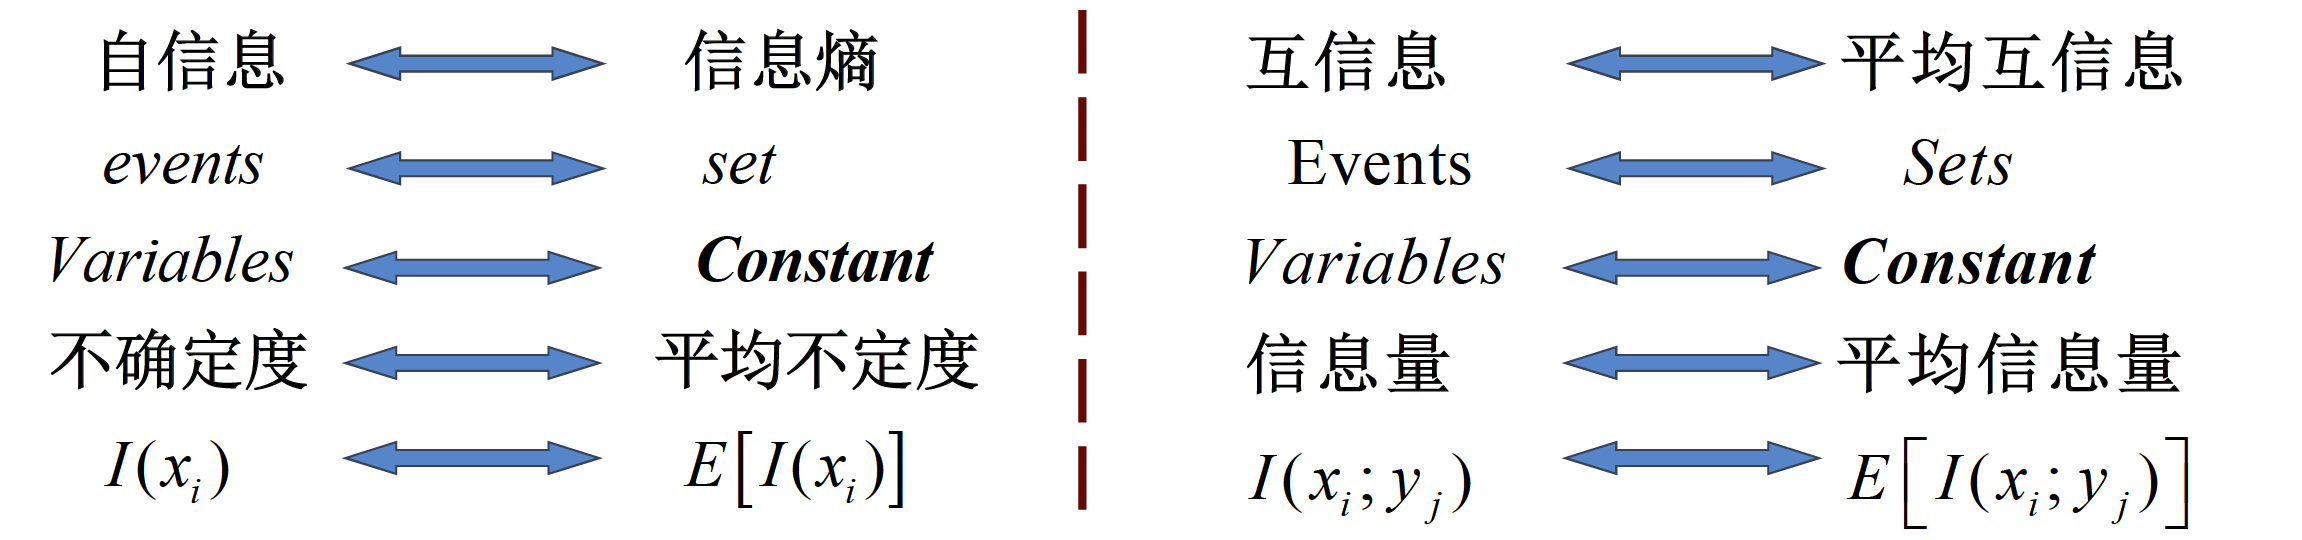
\includegraphics[width=0.9\textwidth]{./figure/fig1.png}
    \end{figure}
    性质:\begin{itemize}
        \item 非负性,即 $I(X; Y)\ge 0$。该性质表明,通过一个信道总能传递一些信息, 最差的条件下,输入输出完全独立,不传递任何信息,平均互信息等于 $0$, 但决不会失去己知的信息
        \item 对称性,即$I(X; Y)=I(Y; X)$。$I(Y; X)$表示从 $X$ 中提取关于的 $Y$ 的信息量,实际上 $I(X; Y)$ 和 $I(Y; X)$只是观察者的立足点不同,对信道的输入 $X$ 和输出 $Y$ 的总体测度的两种表达形式
        \item 极值性,即 $I(X; Y)\le H(X)$。一般来说,平均互信息总是小于信源的熵,只有当信道是无损信道时,平均互信息才等于信源的熵率。
        \item 凸状性,$I(X; Y)$是二元函数:$P(X)$ 的上凸函数,$P(Y/X)$ 的下凸函数。\[I(X ; Y)=\sum_{i} \sum_{j} p(x_{i} y_{j}) \log \frac{p(y_{j} / x_{i})}{p(y_{j})}, p(x_{i} y_{j})=p(x_{i}) p(y_{j} / x_{i}), p(y_{j})=\sum_{i} p(x_{i} y_{j})\]
        \item 对于固定的信道,平均互信息 $I(X; Y)$ 是信源概率分布 $P(X)$ 的上凸函数
        \item 对于固定的信源,平均互信息 $I(X; Y)$ 信道传递概率分布 $P(Y / X)$ 的下凸
        函数
    \end{itemize}
    \begin{figure}[htbp]
        \centering
        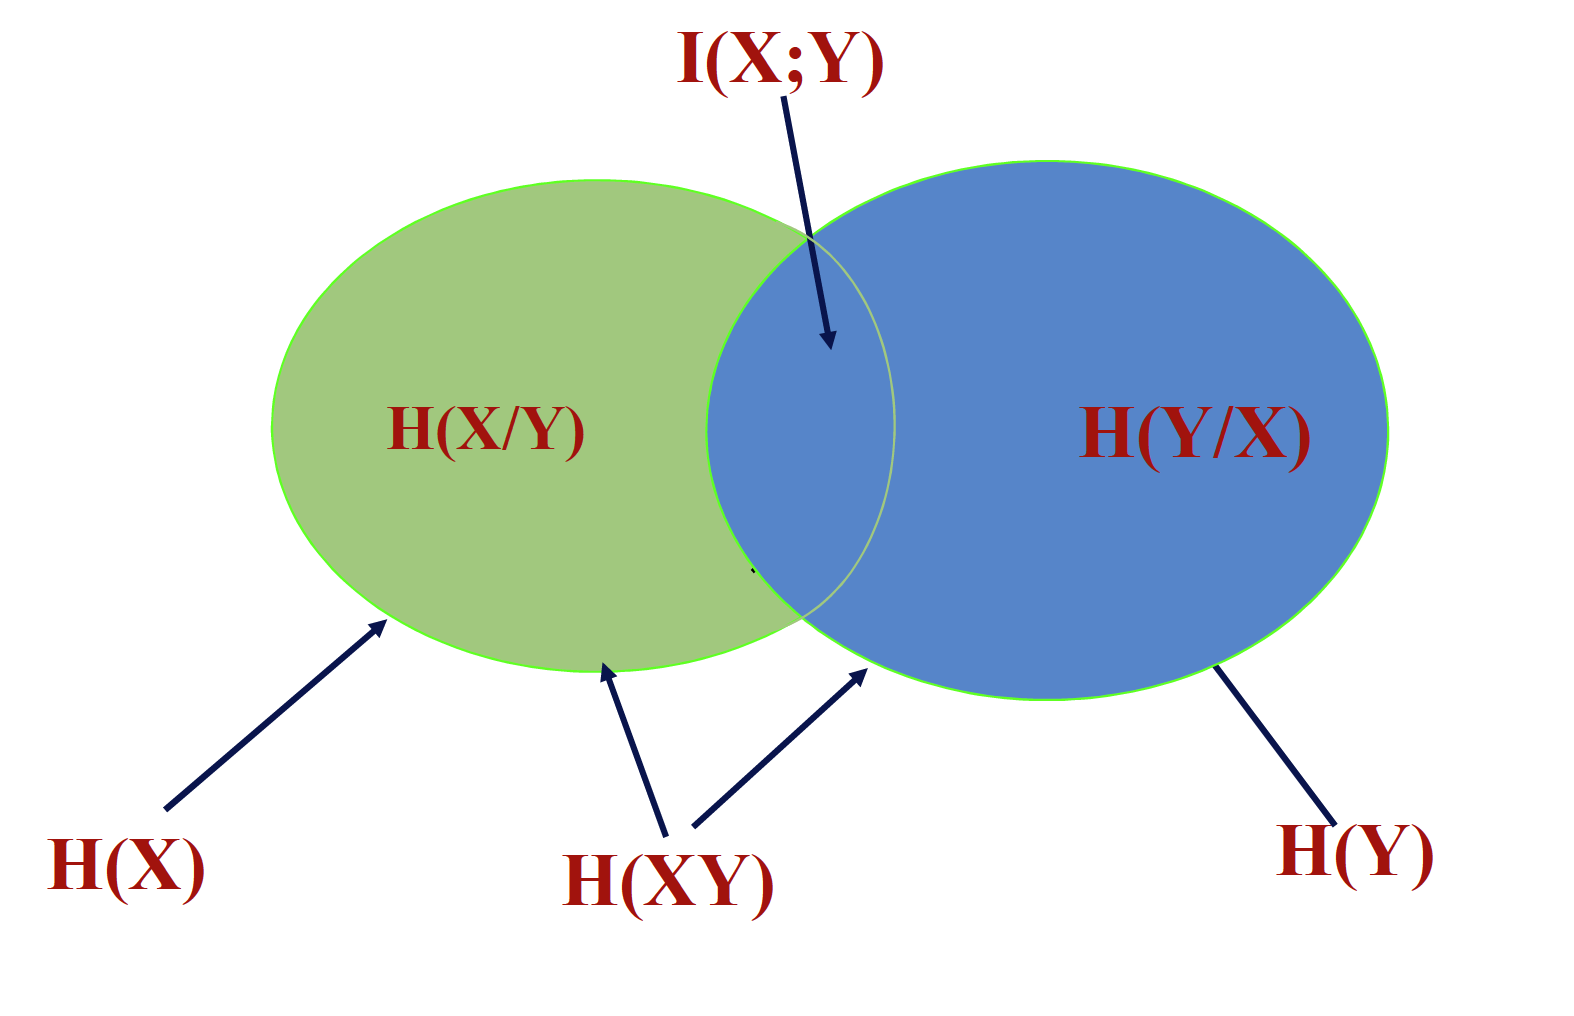
\includegraphics[width=0.5\textwidth]{./figure/fig2.png}
        \caption{平均互信息与熵之间的关系}
    \end{figure}
\end{remark}

\begin{remark}
    互信息的应用:
    \begin{itemize}
        \item 信息不可增性原理:$X$ 经过处理得到 $Y$,$Y$ 经过处理得到 $Z$,有 $I(X; Z) \le I(X; Y)$。不触及源端的处理,每经一次处理,总会丢失信息,最多保持原有的信息不变。
        \item 测试系统中的互信息:$I(X; Y_1) \le I(X; Y_1Y_2) \le \cdots \le I(X; Y_1\cdots Y_m)$。若想通过测试系统来获取源端信息,即从测量的结果 $Y$ 中获得关于 $X$ 的信息,要想多得信息,必须多付出代价,如采用多次测量法。
    \end{itemize}
\end{remark}

\begin{remark}
    如果把 $p(x)$ 和 $q(x)$ 定义在同一概率空间上的两种概率测度,则定义 $p$ 相对于 $q$ 的信息散度为:\[D(p//q) = \sum_Xp(x)\log\frac{p(x)}{q(x)}\]其中$\underset{X}{\sum}p(x) = 1, \underset{X}{\sum}q(x) = 1$
    \begin{itemize}
        \item 信息散度又称为相对熵、鉴别信息、方向散度、KL距离等,它是两个概率分布函数 $p$ 和 $q$ 之间“差别”的一种度量。
        \item 不满足对称性,不满足三角不等式,所以叫散度。\[D(p//q) \neq D(q//p), \quad D(p//q) \nleq D(r//p) + D(q//r)\]
    \end{itemize}
\end{remark}

\section{组合优化}
\begin{remark}
    给定一个图 $G(V, E)$\begin{itemize}
        \item 欧拉回路:找一个每条边只走一次的回路,多项式时间复杂度可解
        \item 哈密顿回路:找一个每个点只走一次的回路,多项式时间复杂度不可解
        \item 找一个最小的边集覆盖每个点,最大二分匹配,多项式时间复杂度可解
        \item 找一个最小的点集覆盖每条边,多项式时间复杂度不可解
    \end{itemize}
\end{remark}

\begin{remark}
    优化问题描述转换为决策问题描述:
    \begin{itemize}
        \item 优化问题:$\langle I = \left\{G=(V, E), u \to v \text{最短路是什么}\right\},S = \{G=(V, E), u \to v \text{最短路}\}\rangle$
        \item 决策问题:$\langle I^\prime = \left\{G=(V, E) \text{是否存在一条从} u \text{到} v \text{长度最少为} k \text{的最短路}\right\} \rangle$
    \end{itemize}
\end{remark}

\begin{remark}
    \text{}
    \begin{itemize}
		\item P问题:多项式时间复杂度可解。
		\item NP问题:多项式时间复杂度可验证。
		\item NP-Complete:没有找到多项式时间复杂度解决算法,可以在多项式时间复杂度内验证。
		\item NP-Hard:没有找到多项式时间复杂度解决算法,并且不可在多项式时间复杂度内验证。
        \item 如果有一个NPC问题在多项式时间复杂度内可解,则P=NP。
        \item 如果存在NP不是多项式时间可解的问题,则没有NPC问题是多项式时间可解的。
    \end{itemize}
\end{remark}

\begin{remark}
    \textbf{证明问题L是NP完全问题}\begin{enumerate}
        \item $L \in NP$
        \item 找到一个 NPC 问题 $L^\prime$
        \item 把 $L^\prime$ 问题规约到 $L$ 问题($L^\prime \le L$),需要 $L$ 问题为真推 $L^\prime$ 问题为真,$L^\prime$ 为真推 $L$ 问题为真。
        \item 说明转换 $f$ 是多项式时间的
    \end{enumerate}
\end{remark}

\begin{remark}
    NPC 问题\begin{itemize}
        \item 第一个NPC问题:电路可满足性问题,给定一个电路,电路由输入节点、与输入节点在同一层的常数节点、与或非节点构成的电路。 是否存在一个输入,使得输出为 $1$。\begin{itemize}
            \item CIRCUIT-SAT = $\left\{<C>:C\text{是一个可满足的电路}\right\}$
        \end{itemize}
        \begin{figure}[htbp]
            \centering
            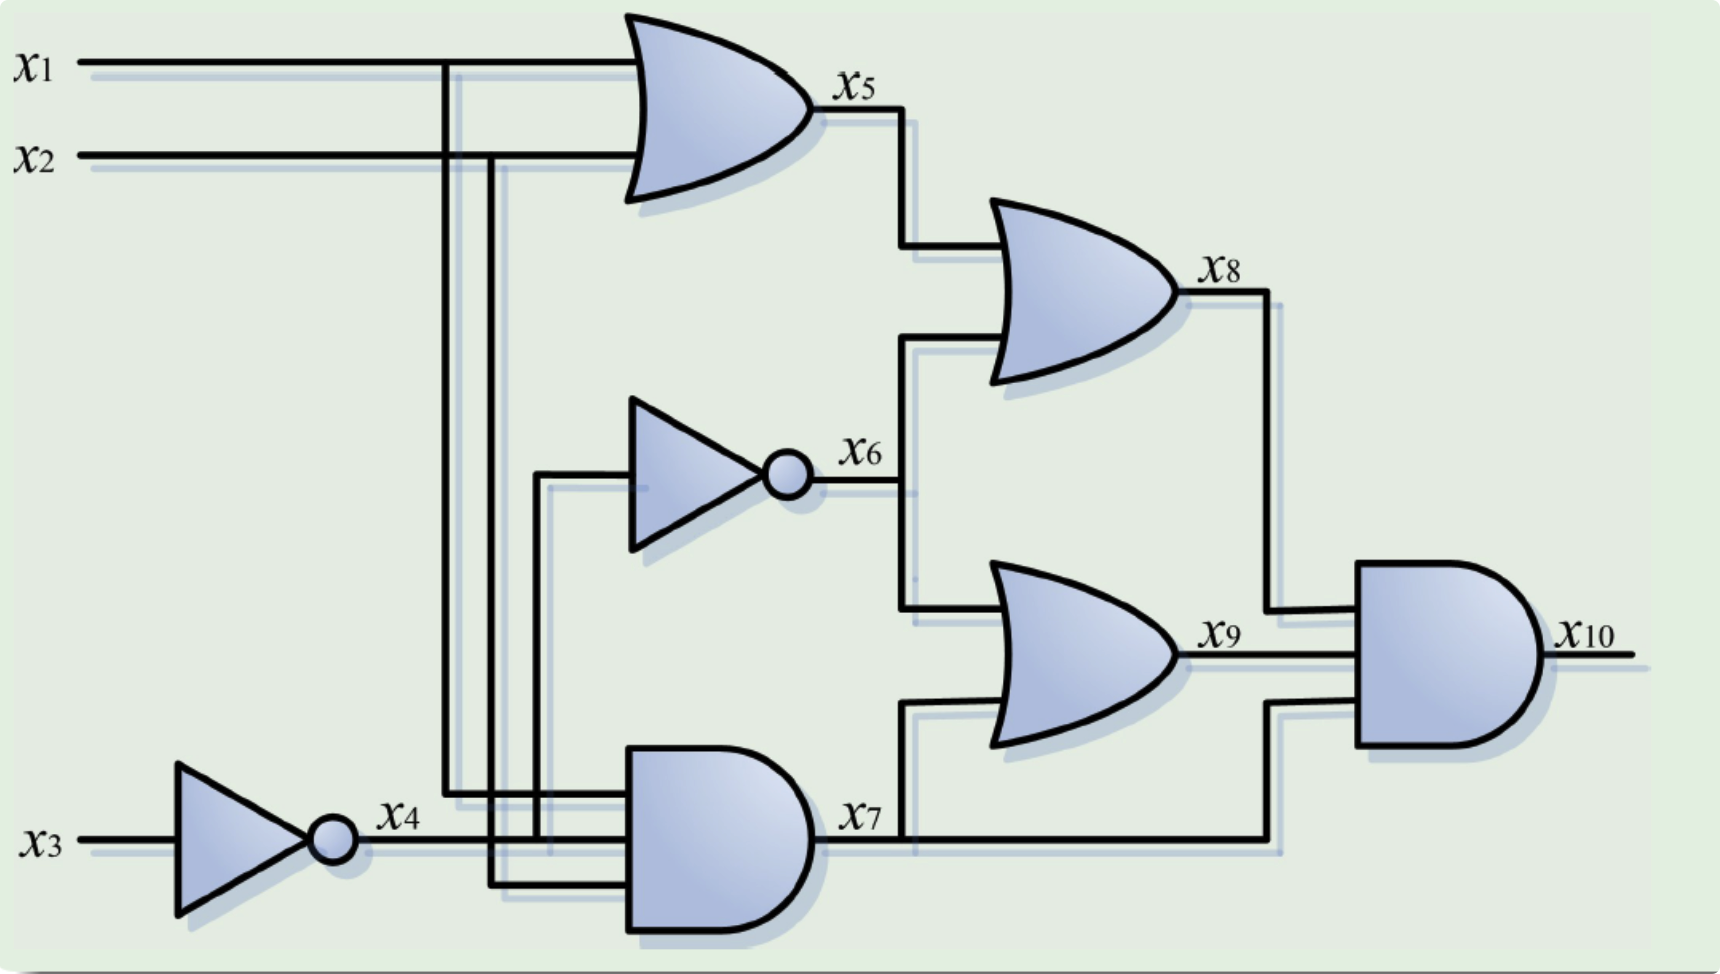
\includegraphics[width=0.5\textwidth]{./figure/fig3.png}
        \end{figure}
        \item SAT = $\left\{<f>, f\text{是一个可满足的布尔表达式}\right\}$
        \begin{figure}[htbp]
            \centering
            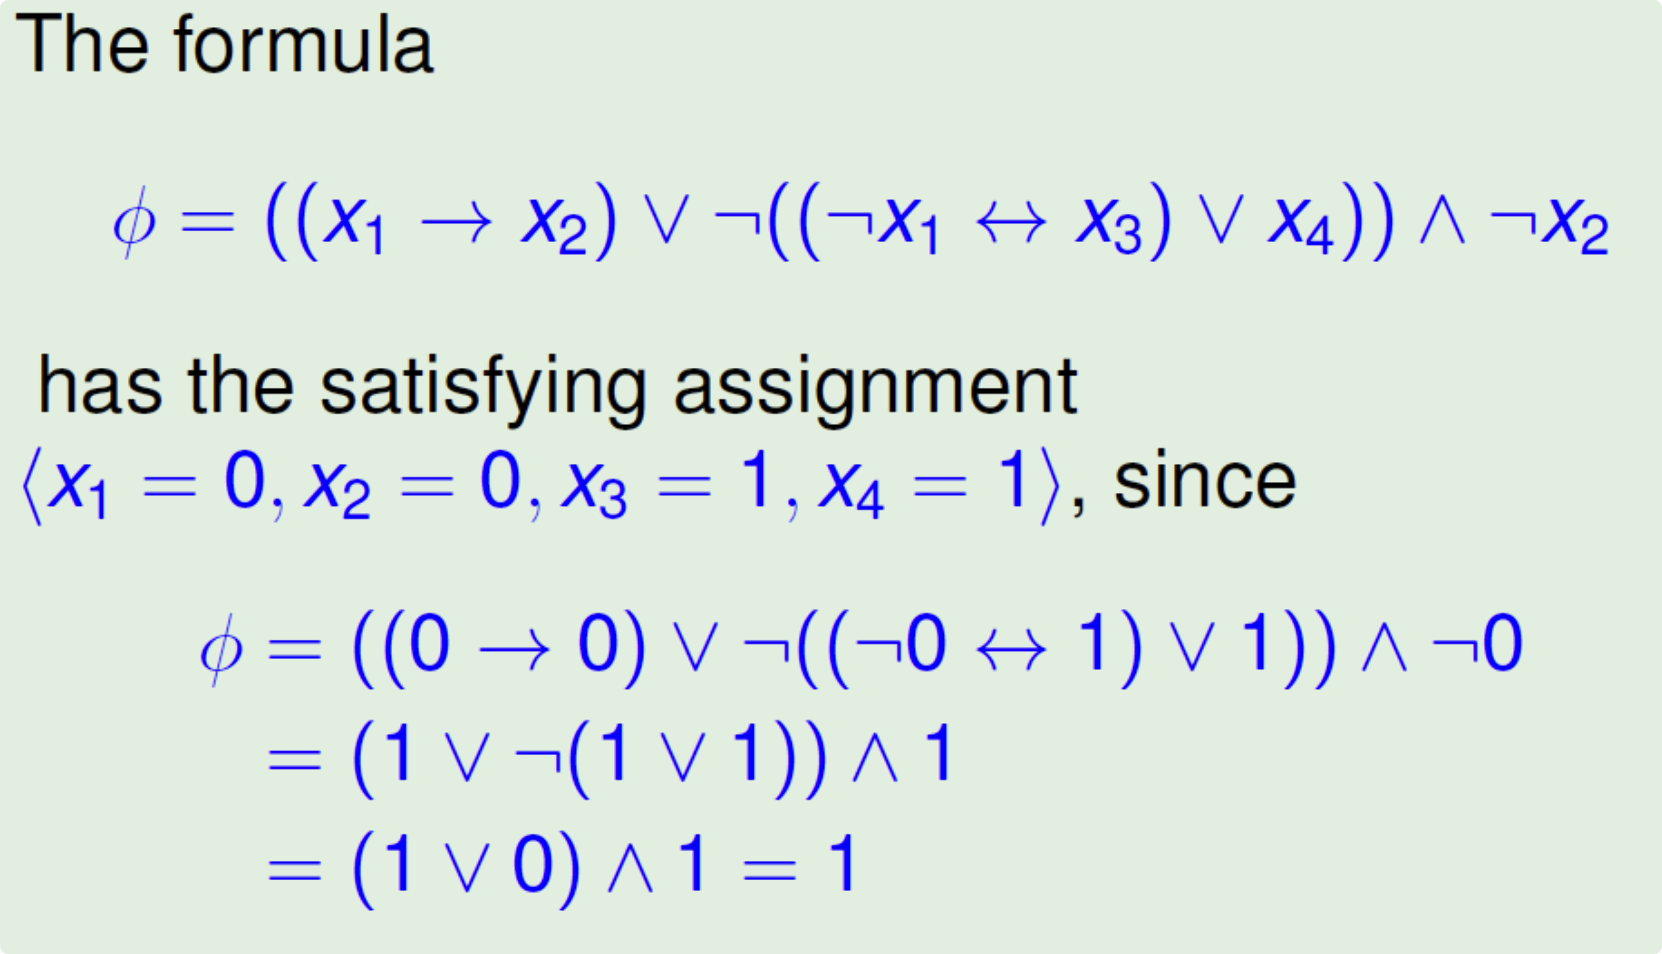
\includegraphics[width=0.5\textwidth]{./figure/fig4.png}
        \end{figure}
        \item 旅行商问题:$\left\{<G, c, k>: G=(V, E)\text{是一个完全图,}c\text{是边权}\right.$,存在一个哈密顿回路使得边权总和不大于 $k\left.\right\}$
    \end{itemize}
\end{remark}

\begin{remark}
    使用近似算法得到计算结果 $C$,最佳结果 $C^\prime$,近似度等于 $\max(\frac{C}{C^\prime}, \frac{C^\prime}{C}) \ge 1$。
\end{remark}


\section{博弈论}
\begin{remark}
    概念理解:
    \begin{itemize}
        \item 马尔可夫博弈(或随机博弈)是机器学习中多智能体强化学习的理论基础。
        \item 常和博弈:两个博弈者的每轮收益和是常数。
        \item 零和博弈:纯竞争博弈。零和博弈表示所有博弈方的利益之和为零或一个常数,即一方有收入,其他方必有所失,如猜拳游戏。
        \item 正则型博弈:用矩阵描述博弈。
        \item 扩展型博弈:通过树来描述博弈。博弈从唯一的初始节点开始,通过由参与者决定的路径到达终端节点,参与者得到相应的收益。和正则形式不同,扩展形式允许互动的显式模型,互动中,一个参与者可以在博弈中多次行动,并且在不同的状态中可以做出不同的行为。
        \item 帕累托最优:没有办法在不让某一参与资源分配的一方利益受损的情况下,令另一方获得更大利益的。例如囚徒困境(数值越小越好):图中绿色圈的是帕累托最优,$(1, 1)$ 严格比 $(5, 5)$ 更优。
        \begin{figure}[htbp]
            \centering
            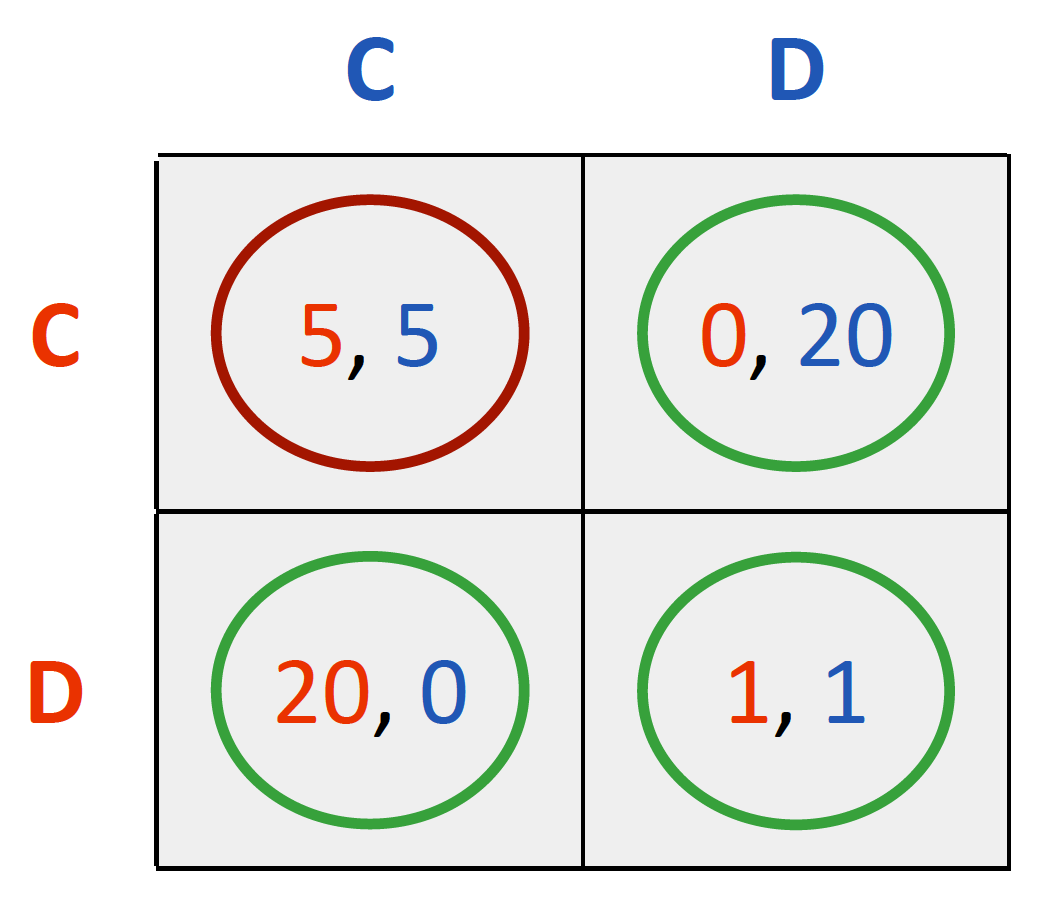
\includegraphics[width=0.4\textwidth]{./figure/fig5.png}
        \end{figure}
        \item 纳什均衡:没有参与者可以透过改变自身策略使自身受益时的一个概念解。例如猎鹿赛局(数值越大越好):途中红色圈都是纳什均衡解,绿色圈是稳定的纳什均衡解。
        \begin{figure}[htbp]
            \centering
            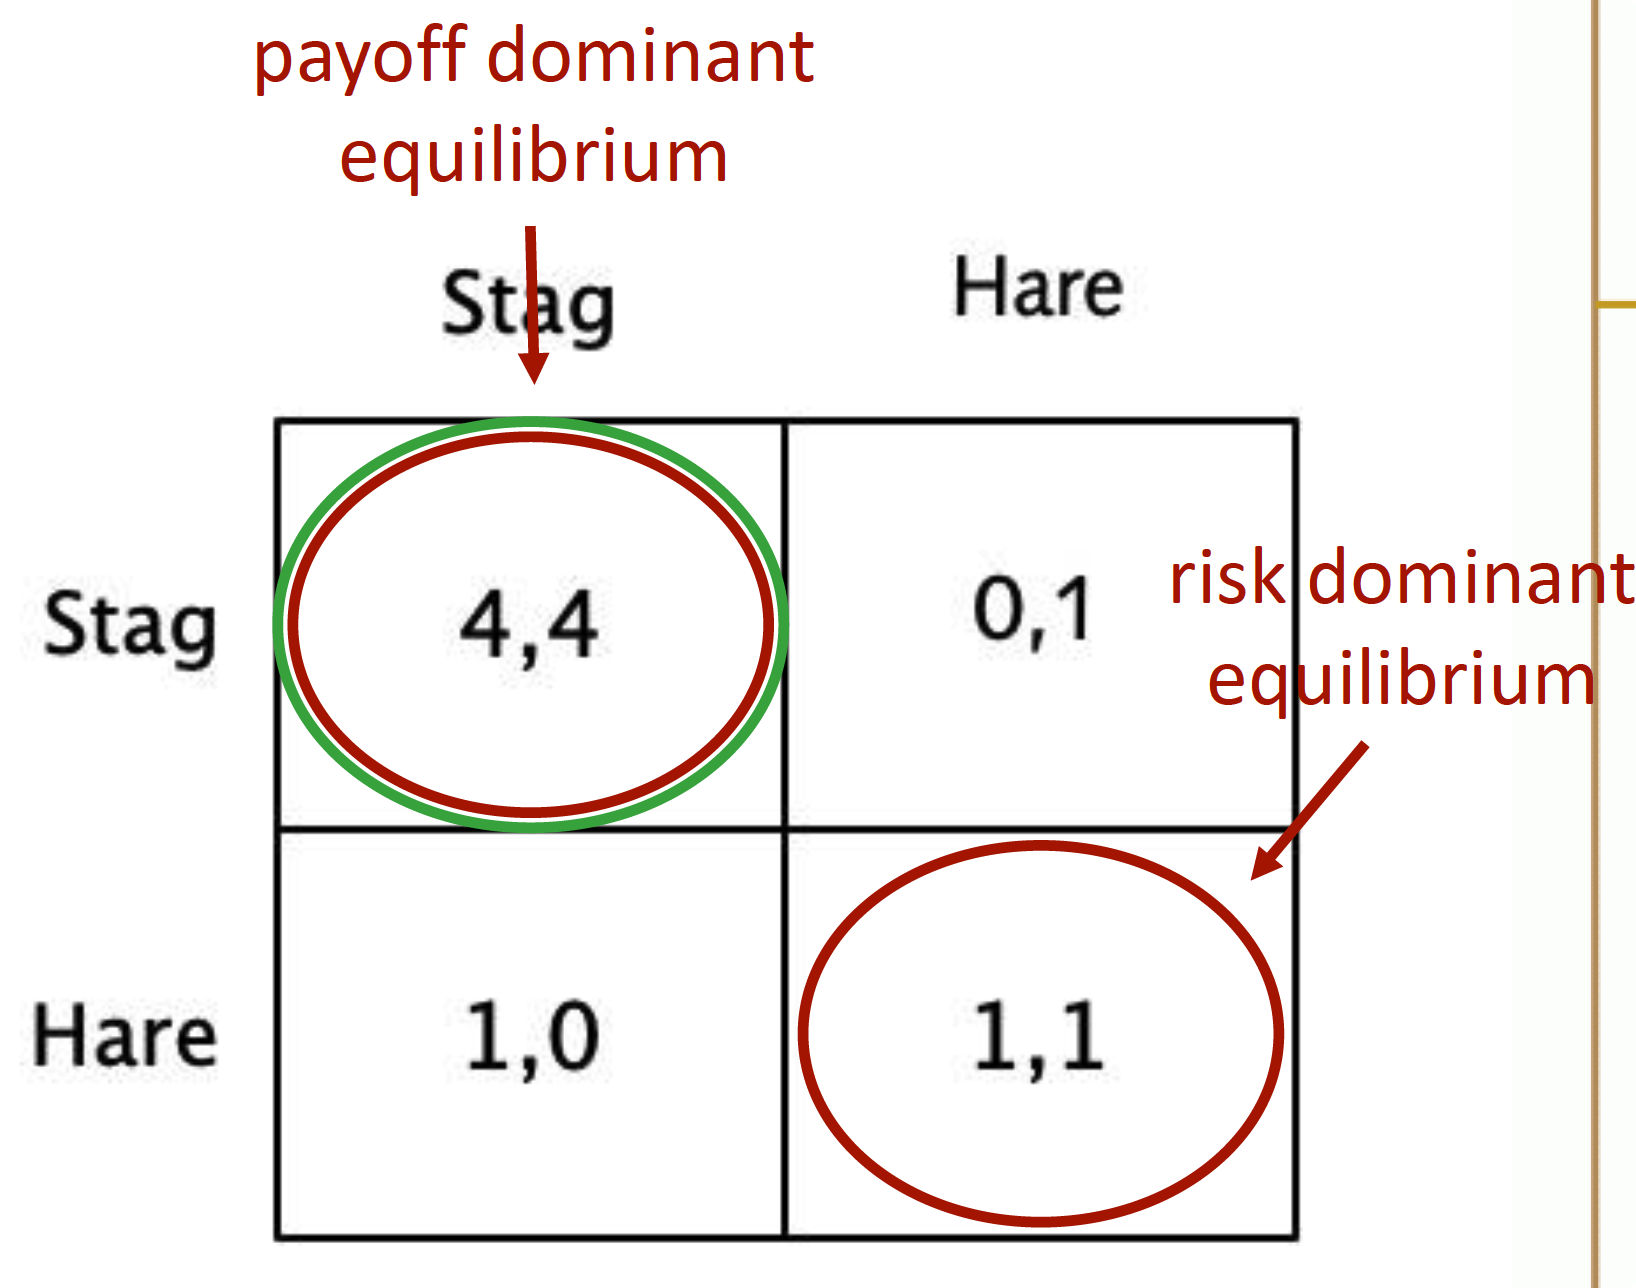
\includegraphics[width=0.4\textwidth]{./figure/fig6.png}
        \end{figure}
        \item 并不是所有的博弈都存在纯策略纳什均衡,但是至少存在一个混合策略纳什均衡。
        \item 对于扩展式博弈的策略组合,如果它是原博弈的纳什均衡,并且在每一个子博弈上也都构成纳什均衡,则它是一个子博弈精炼纳什均衡。子博弈精炼均衡是比纳什均衡更强的概念。
        \item 完美信息博弈一定存在纯策略纳什均衡。
        \item 不完全博弈不知道自己在进行什么博弈游戏,不完美博弈不知道自己处于哪个状态(博弈树的节点)。不完全信息博弈中的不确定性比不完美信息博弈中的不确定性要高。
    \end{itemize}
\end{remark}

\begin{remark}
    性别之战:夫妻看电影
    \begin{figure}[htbp]
        \centering
        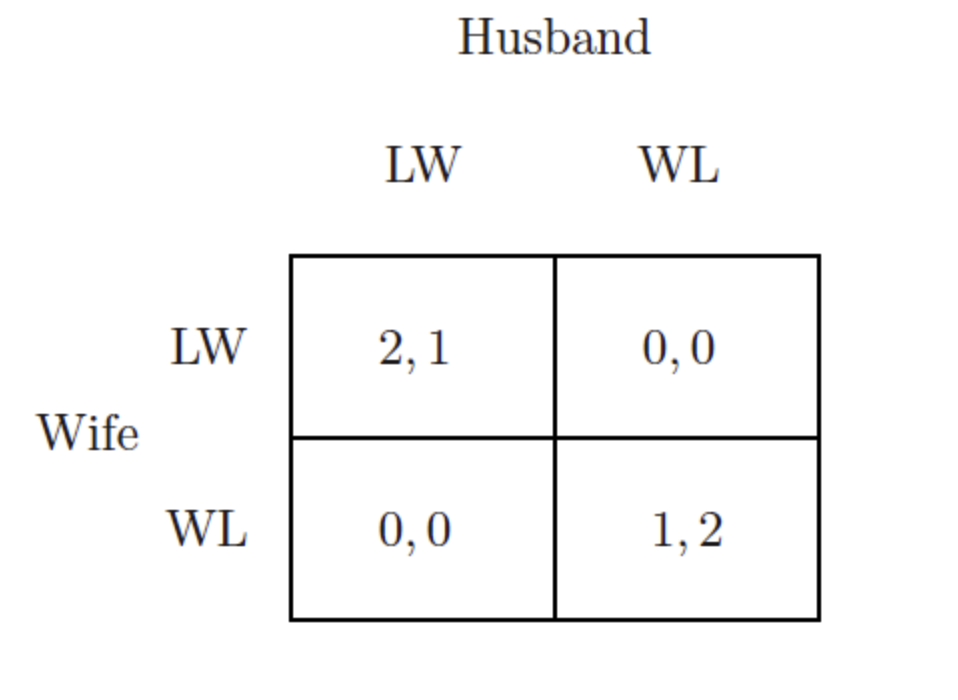
\includegraphics[width=0.4\textwidth]{./figure/fig7.png}
        \caption{性别之战}
    \end{figure}
    \begin{enumerate}
        \item 两个纯策略纳什均衡解
        \item 混合策略纳什均衡\begin{itemize}
            \item 假设丈夫的策略是以概率 $p$ 选LW,以概率 $1-p$ 选WL
            \item 妻子不知道丈夫的两个行动 \begin{align*}
                U_{\text{wife}}(LW) &= U_{\text{wife}}(WL)\\
                2\cdot p + 0 \cdot (1 - p) &= 0 \cdot p + 1 \cdot (1 - p)
            \end{align*}
            \item 可得丈夫的策略:1 / 3选LW, 2 / 3 选WL。
            \item 同理妻子的策略:2 / 3 选LW, 1 / 3 选WL。
            \item 如果混合策略是最好的,那么混合中涉及的每一种纯策略本身就一定是最佳。也就是,每一项都必须产生相同的预期回报。
        \end{itemize}
    \end{enumerate}
\end{remark}

\begin{remark}
    alpha-beta剪枝(\href{https://oiwiki.org/search/alpha-beta/}{参考资料}) 
    \lstinputlisting[style=cpp]{./alpha-beta.cpp}
    \begin{figure}[htbp]
        \centering
        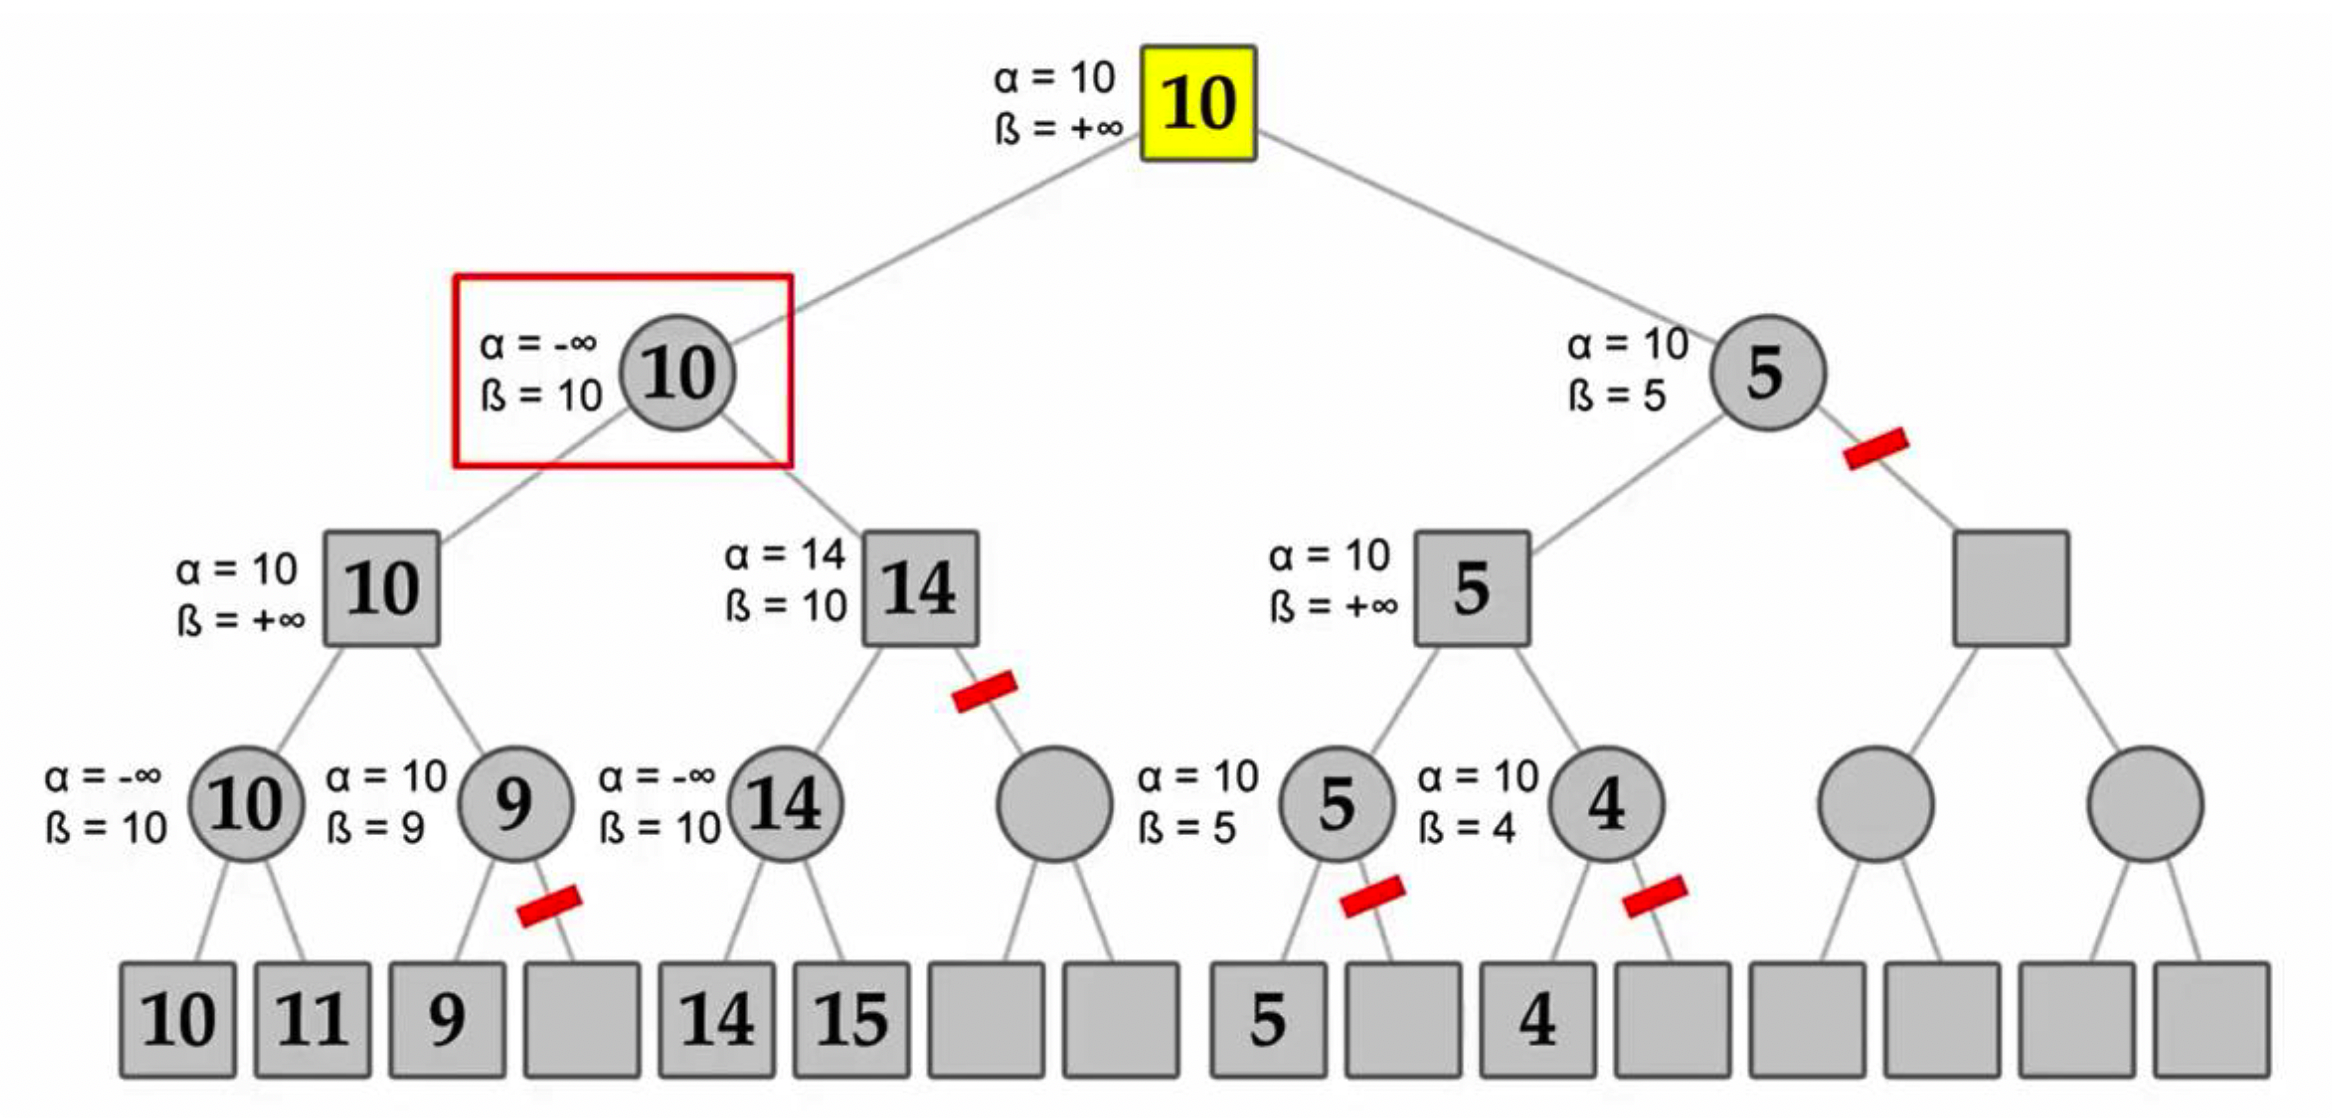
\includegraphics[width=0.8\textwidth]{./figure/fig8.png}
        \caption{alpha-beta 剪枝 \label{fig8}}
    \end{figure}
\end{remark}

\begin{remark}
    扩展型博弈与正则型博弈转换
    \begin{itemize}
        \item 选数,数越大收益越高,完美信息博弈,如图\ref{fig10}
        \begin{figure}[htbp]
            \centering
            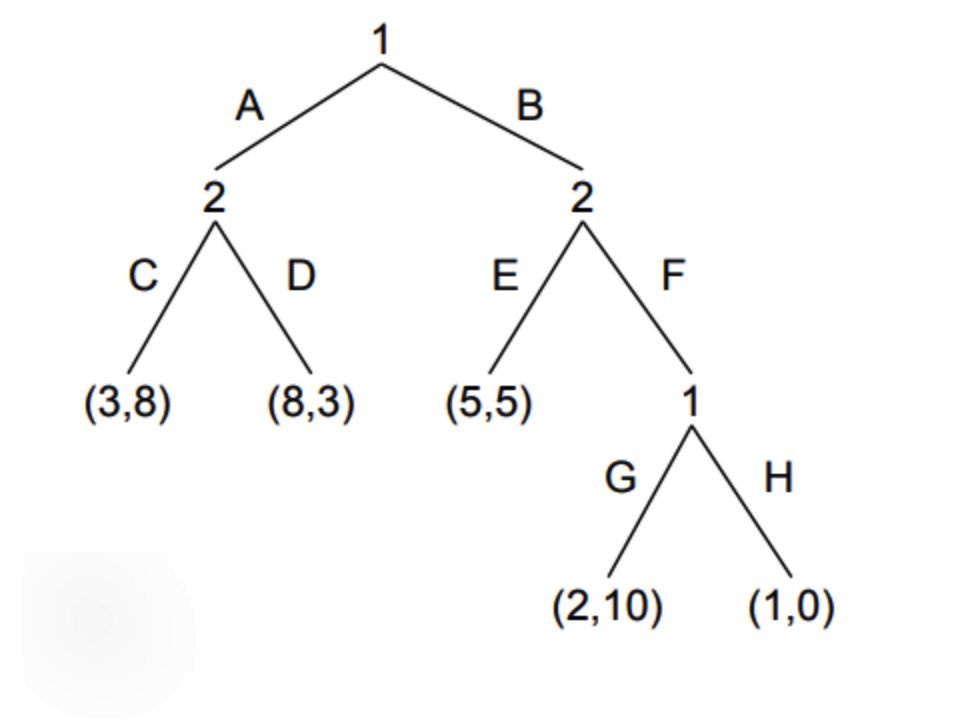
\includegraphics[width=0.4\textwidth]{./figure/fig9.png}
            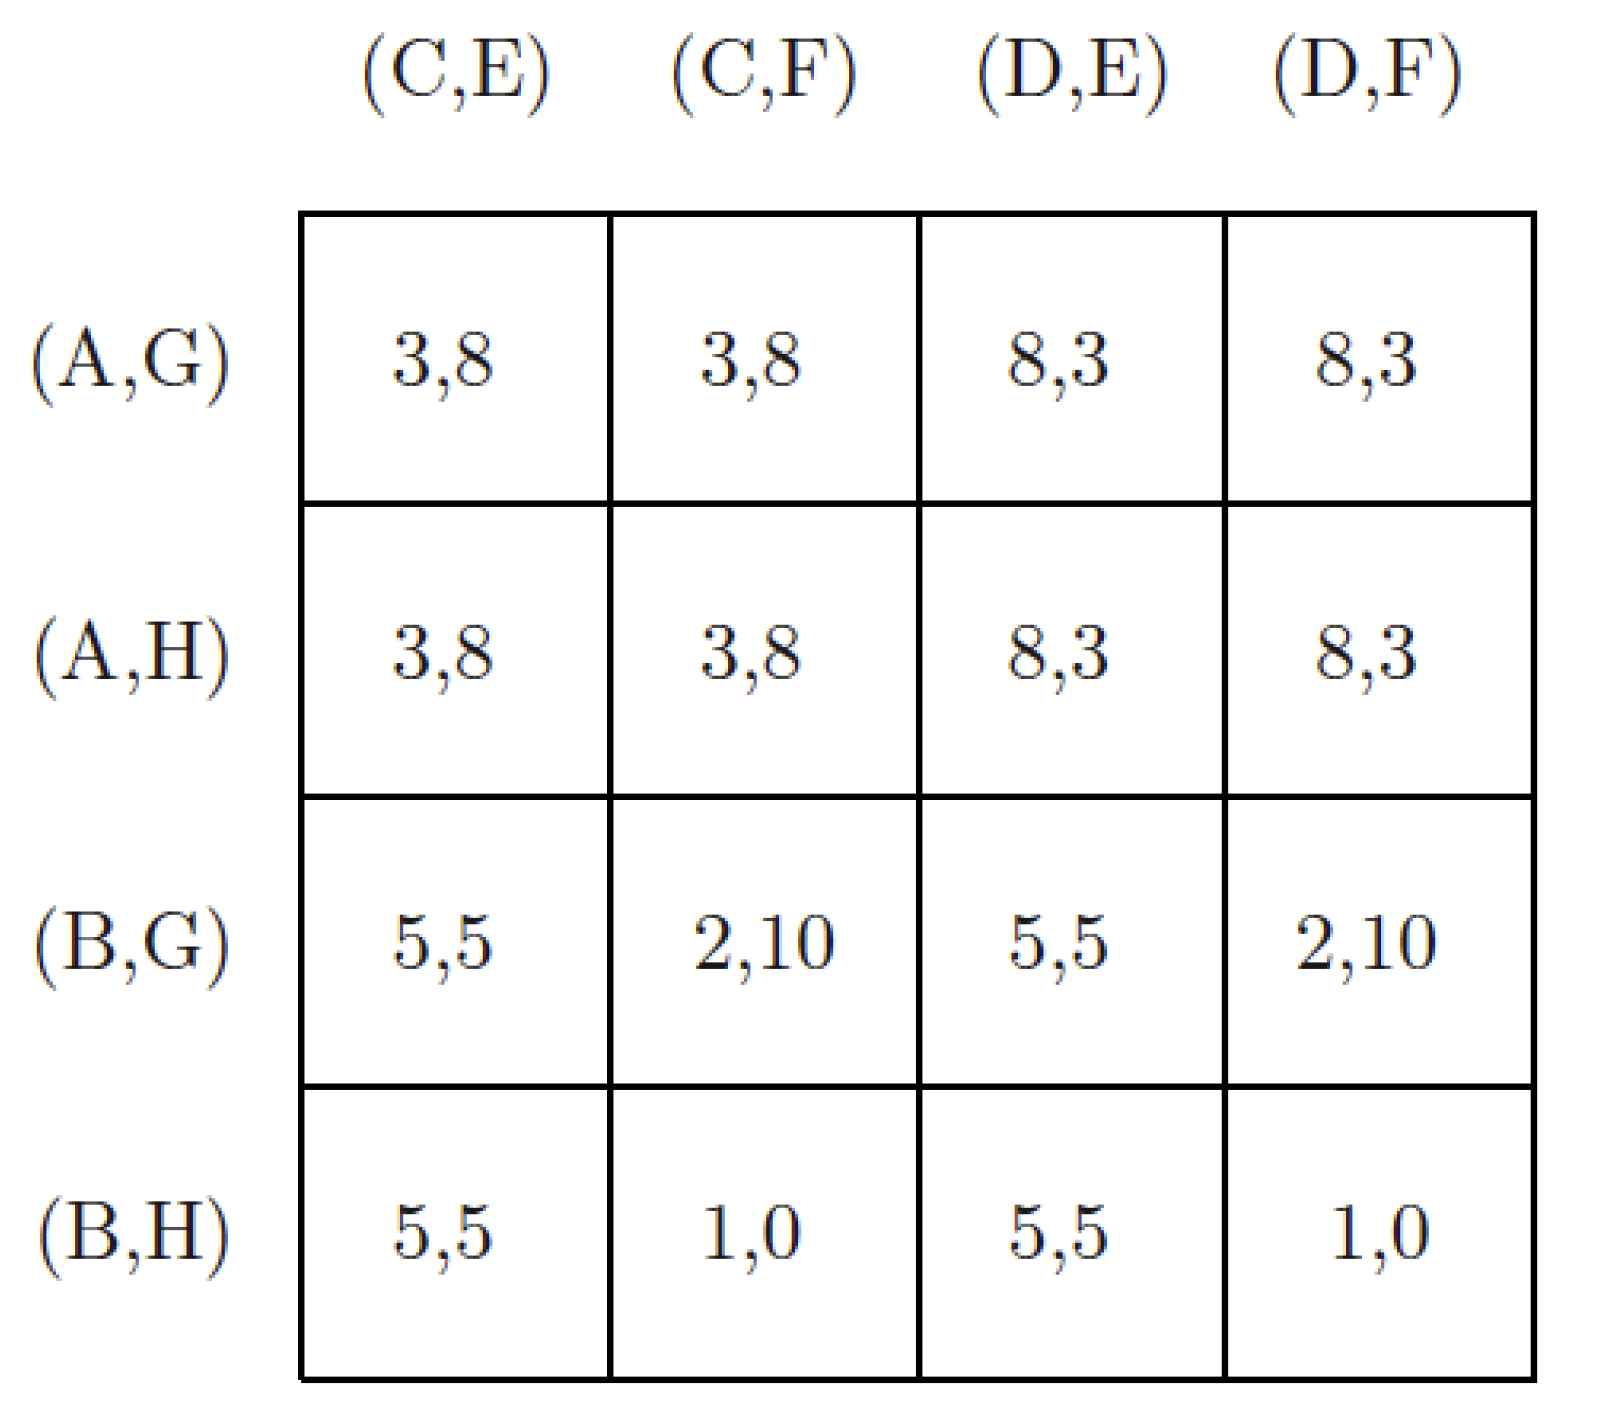
\includegraphics[width=0.4\textwidth]{./figure/fig10.png}
            \caption{扩展型博弈转换为正则型博弈\label{fig10}}
        \end{figure}
        \item 囚徒困境,不完美信息博弈,虚线将属于同一信息集的所有决策结连接起来。此时决策者不知道自己处于哪一个点,可能处于虚线连接的任何一个点。如图\ref{fig11}
        \begin{figure}[htbp]
            \centering
            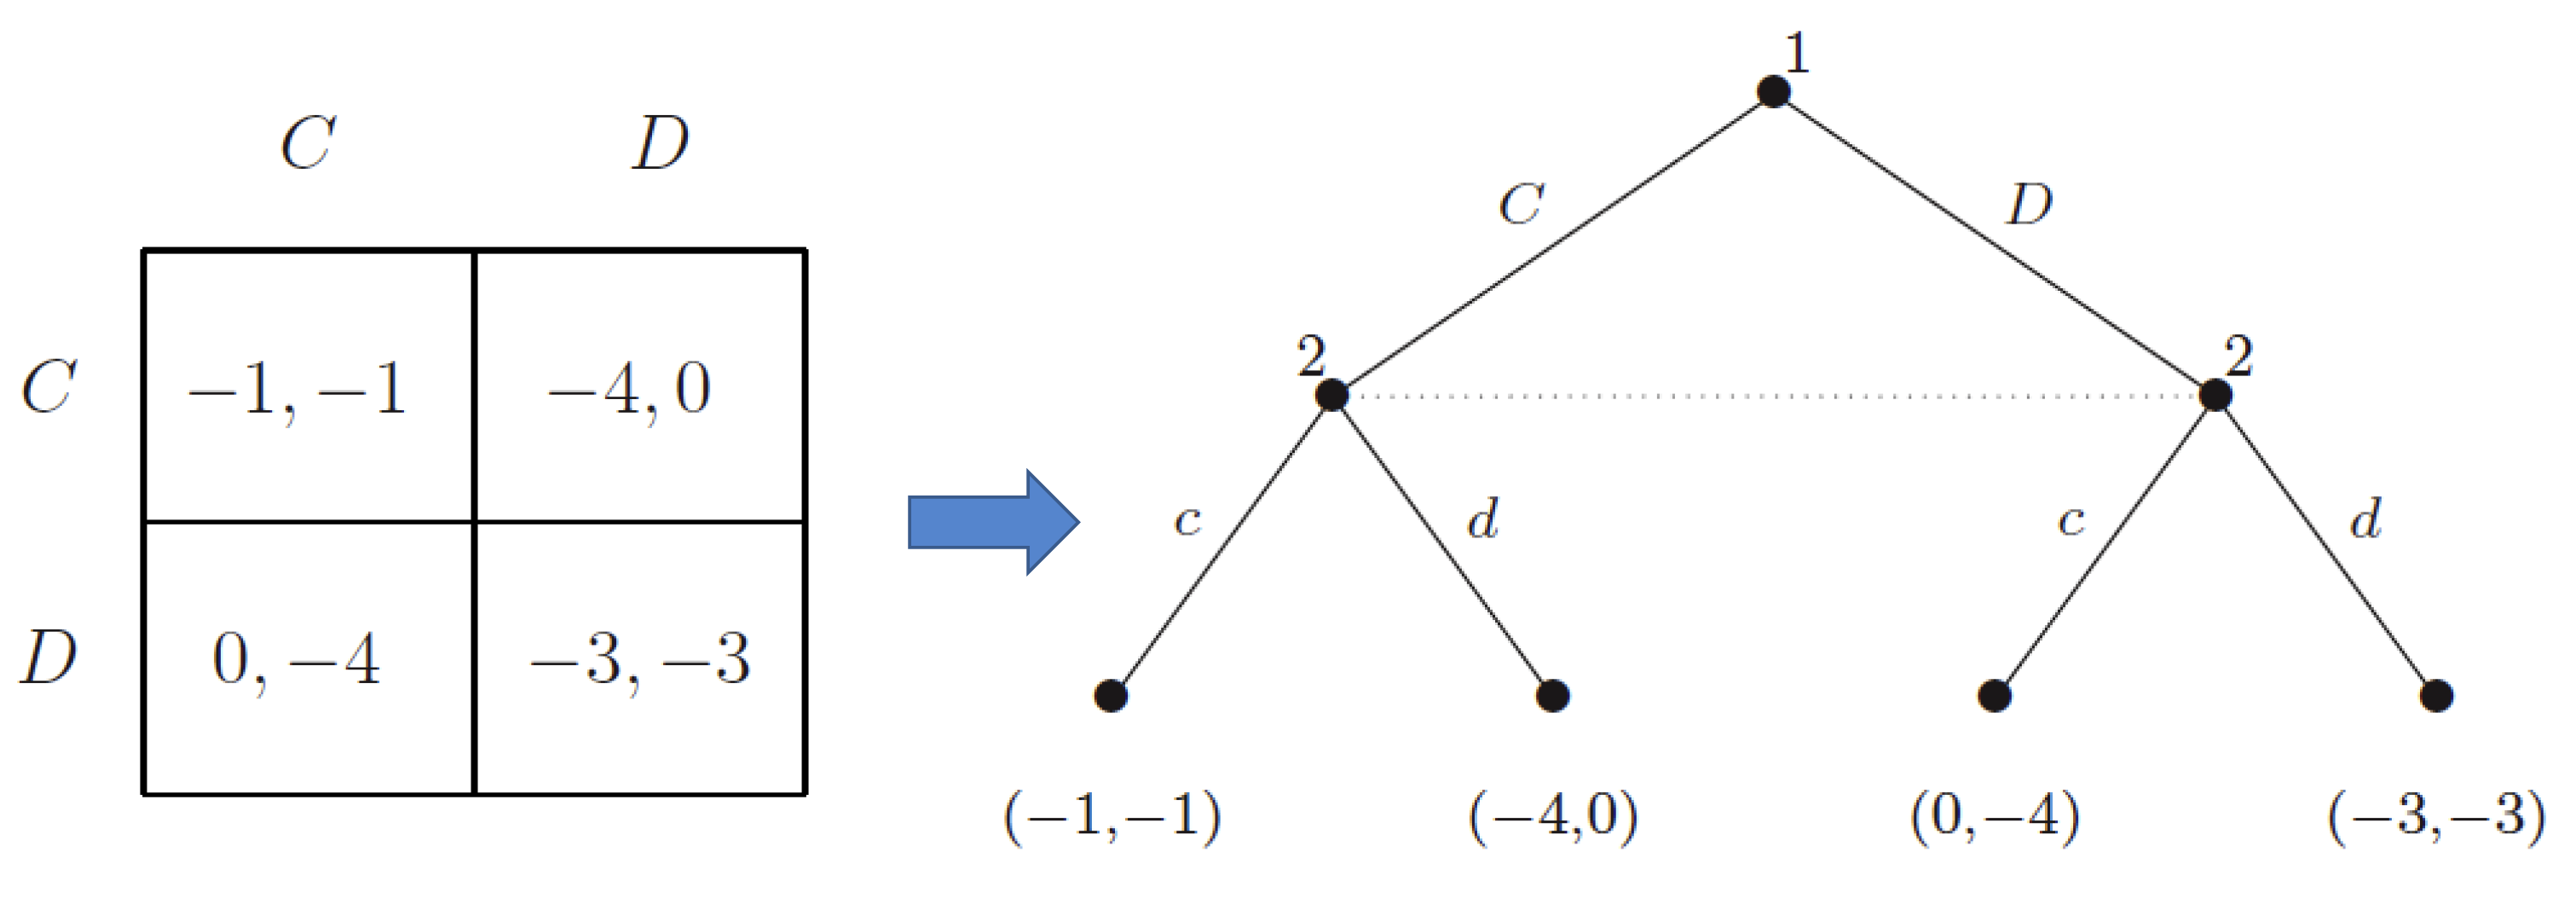
\includegraphics[width=0.8\textwidth]{./figure/fig11.png}
            \caption{扩展型博弈转换为正则型博弈\label{fig11}}
        \end{figure}
    \end{itemize}
\end{remark}


\end{document}